\appendix
\section*{Anhang}
\appendixtoc
\captionsetup{listof=false}
\clearpage

\begin{landscape}
\section{Anforderungen}
\subsection{Vollständige Anforderungsliste}

\small
\setlength{\tabcolsep}{3pt}
\renewcommand{\arraystretch}{1.15}
\setlength{\LTcapwidth}{\textwidth}
\captionsetup{justification=raggedright,singlelinecheck=false}

\begin{longtable}{|l|p{2,2cm}|p{8.5cm}|l|l|l|l|l|p{4.0cm}|}

\hline
\textbf{ID} &
\textbf{Kategorie} &
\textbf{Anforderung} &
\textbf{Wert} &
\textbf{Einheit} &
\textbf{Priorität} &
\textbf{Datum} &
\textbf{Status} &
\textbf{Kommentar} \\
\hline
\endfirsthead

\hline
\textbf{ID} &
\textbf{Kategorie} &
\textbf{Anforderung} &
\textbf{Wert} &
\textbf{Einheit} &
\textbf{Priorität} &
\textbf{Datum} &
\textbf{Status} &
\textbf{Kommentar} \\
\hline
\endhead
\endlastfoot

A01 & Funktional &
Das System muss mit den vorhandenen Werkstückträgern (WST) kompatibel sein &
— & — & MUSS & 27.06.25 & Erfüllt &
Ermöglicht automatische Bestückung \\
\hline

A02 & Funktional &
Das System muss die Baugrößen SLC-17 und SLC-24 verarbeiten können &
— & — & MUSS & 27.06.25 & Erfüllt &
SLC-17 = SLC mit 17\,mm Breite \\
\hline

A03 & Funktional &
SLC-Positionierer mit Wand (SLC-W) müssen mittels Keile vorgespannt werden können &
— & — & MUSS & 27.06.25 & Erfüllt &
SLC-W = SLC mit Wand \\
\hline

A04 & Funktional &
SLC-Positionierer ohne Wand müssen mit dem bestehenden Vorspannsystem vorgespannt werden &
— & — & MUSS & 27.06.25 & Erfüllt &
— \\
\hline

A05 & Funktional &
Das Vorspannsystem muss das Führungspaket parallel zur Referenzfläche ausrichten. &
$< 20$ & $\mu$m & MUSS & 27.06.25 & Erfüllt &
Gleiche Breite überall \\
\hline

A06 & Funktional &
Die Schrauben sind mit einem vordefinierten Drehmoment anzuziehen &
25 - 60 & $Ncm$ & MUSS & 27.06.25 & Erfüllt &
— \\
\hline

A07 & Funktional &
Das Schraubwerkzeug muss präzise positioniert werden können &
— & — & MUSS & 27.06.25 & Erfüllt &
— \\
\hline

A08 & Steuerung &
Geeignete Steuerungshardware und -software sind auszuwählen &
— & — & MUSS & 27.06.25 & Erfüllt &
— \\
\hline

A09 & Steuerung &
Testskripte zur Validierung der Steuerungsabläufe sind zu entwickeln &
— & — & MUSS & 27.06.25 & Erfüllt &
— \\
\hline

A10 & Zeitvorgabe &
Die Bearbeitungsdauer pro Positionierer soll unter 5 Minuten liegen &
$< 5$ & min & SOLL & 02.07.25 & Erfüllt &
— \\
\hline

A11 & Mechanik &
Die maximale Systemgröße darf 1200 × 760\,mm nicht überschreiten &
1200 × 760 & mm & MUSS & 27.06.25 & Erfüllt &
— \\
\hline

A12 & Daten\-management &
Relevante Prozessdaten sollen erfasst und dokumentiert werden &
— & — & SOLL & 27.06.25 & In Arbeit &
z.\,B. Seriennummer, Drehmoment, Kraft, Prozessstatus \\
\hline

A13 & Rahmen\-bedingung &
Das Projektbudget beträgt maximal 10.000\,€ &
10.000 & € & MUSS & 27.06.25 & Erfüllt &
— \\
\hline

A14 & Mechanik &
Toleranzen der Montagekomponenten müssen eingehalten werden &
— & — & MUSS & 27.06.25 & Erfüllt &
— \\
\hline

A16 & Sicherheit &
Die genaue Position der Schlitten ist stets zu überwachen &
— & — & MUSS & 27.06.25 & Erfüllt &
— \\
\hline

A19 & Reinraum\-kompatibilität &
Die Station soll für den Einsatz in ISO-6-Umgebungen gemäß ISO 14644-1 geeignet sein &
— & — & SOLL & 29.07.25 & In Arbeit &
— \\
\hline

A19b & Mechanik &
Komponenten müssen robust gegenüber Vibration, Verschleiß und Belastung ausgelegt sein &
— & — & SOLL & 27.06.25 & Erfüllt &
— \\
\hline

A20 & Wartung &
Das System soll wartungsarm und wartungsfreundlich gestaltet sein &
— & — & SOLL & 27.06.25 & Erfüllt &
— \\
\hline

A21 & Erweiter\-barkeit &
Das System soll für künftige Erweiterungen (z.\,B. neue Baugrößen) ausgelegt sein &
— & — & SOLL & 27.06.25 & Erfüllt &
— \\
\hline

A22 & Flexibilität &
Die Umrüstung zwischen SLC-17 und SLC-24 (mit/ohne Wand) soll schnell und werkzeuglos sein &
— & — & SOLL & 27.06.25 & Erfüllt &
— \\
\hline

A23 & Validierung &
Alle Subsysteme sollen kalibriert werden &
— & — & SOLL & 27.06.25 & In Arbeit &
— \\
\hline

A24 & Energie\-effizienz &
Der Energieverbrauch des Systems soll optimiert sein &
— & — & KANN & 30.06.25 & In Arbeit &
— \\
\hline

A25 & Transport &
Das System soll auf Rollen stehen oder modular zerlegbar sein &
— & — & KANN & 30.06.25 & Erfüllt &
— \\
\hline

A26 & Mechanik &
Die Positionierabweichung des Schraubwerkzeugs
darf in jede Richtung nicht größer als \qty{15}{\micro\meter} sein. &
$< 15$ & $\mu$m & MUSS & 30.06.25 & Erfüllt &
— \\
\hline

\caption{Vollständige Anforderungsliste des automatisierten Montagesystems}
\label{tab:anforderungsliste}
\end{longtable}
\end{landscape}

\clearpage

\section{Mechanische Konstruktion}
\label{anhang:2d_zeichnungen}

Die folgenden PDF-Dokumente enthalten die 2D-Zeichnungen der im Montagesystem
verwendeten Baugruppen. Die Zeichnungen dienen der ergänzenden Darstellung
des mechanischen Aufbaus und der Stücklistenstruktur. Die Zeichnungen sind in der folgenden Reihenfolge:

\begin{enumerate}
    \item Gesamtbau
    \item Achssystem
    \item Endeffektor (EE)
    \item Werkstückaufnahme
\end{enumerate}

\clearpage

\begin{landscape}
\label{anhang:gesamtbau}
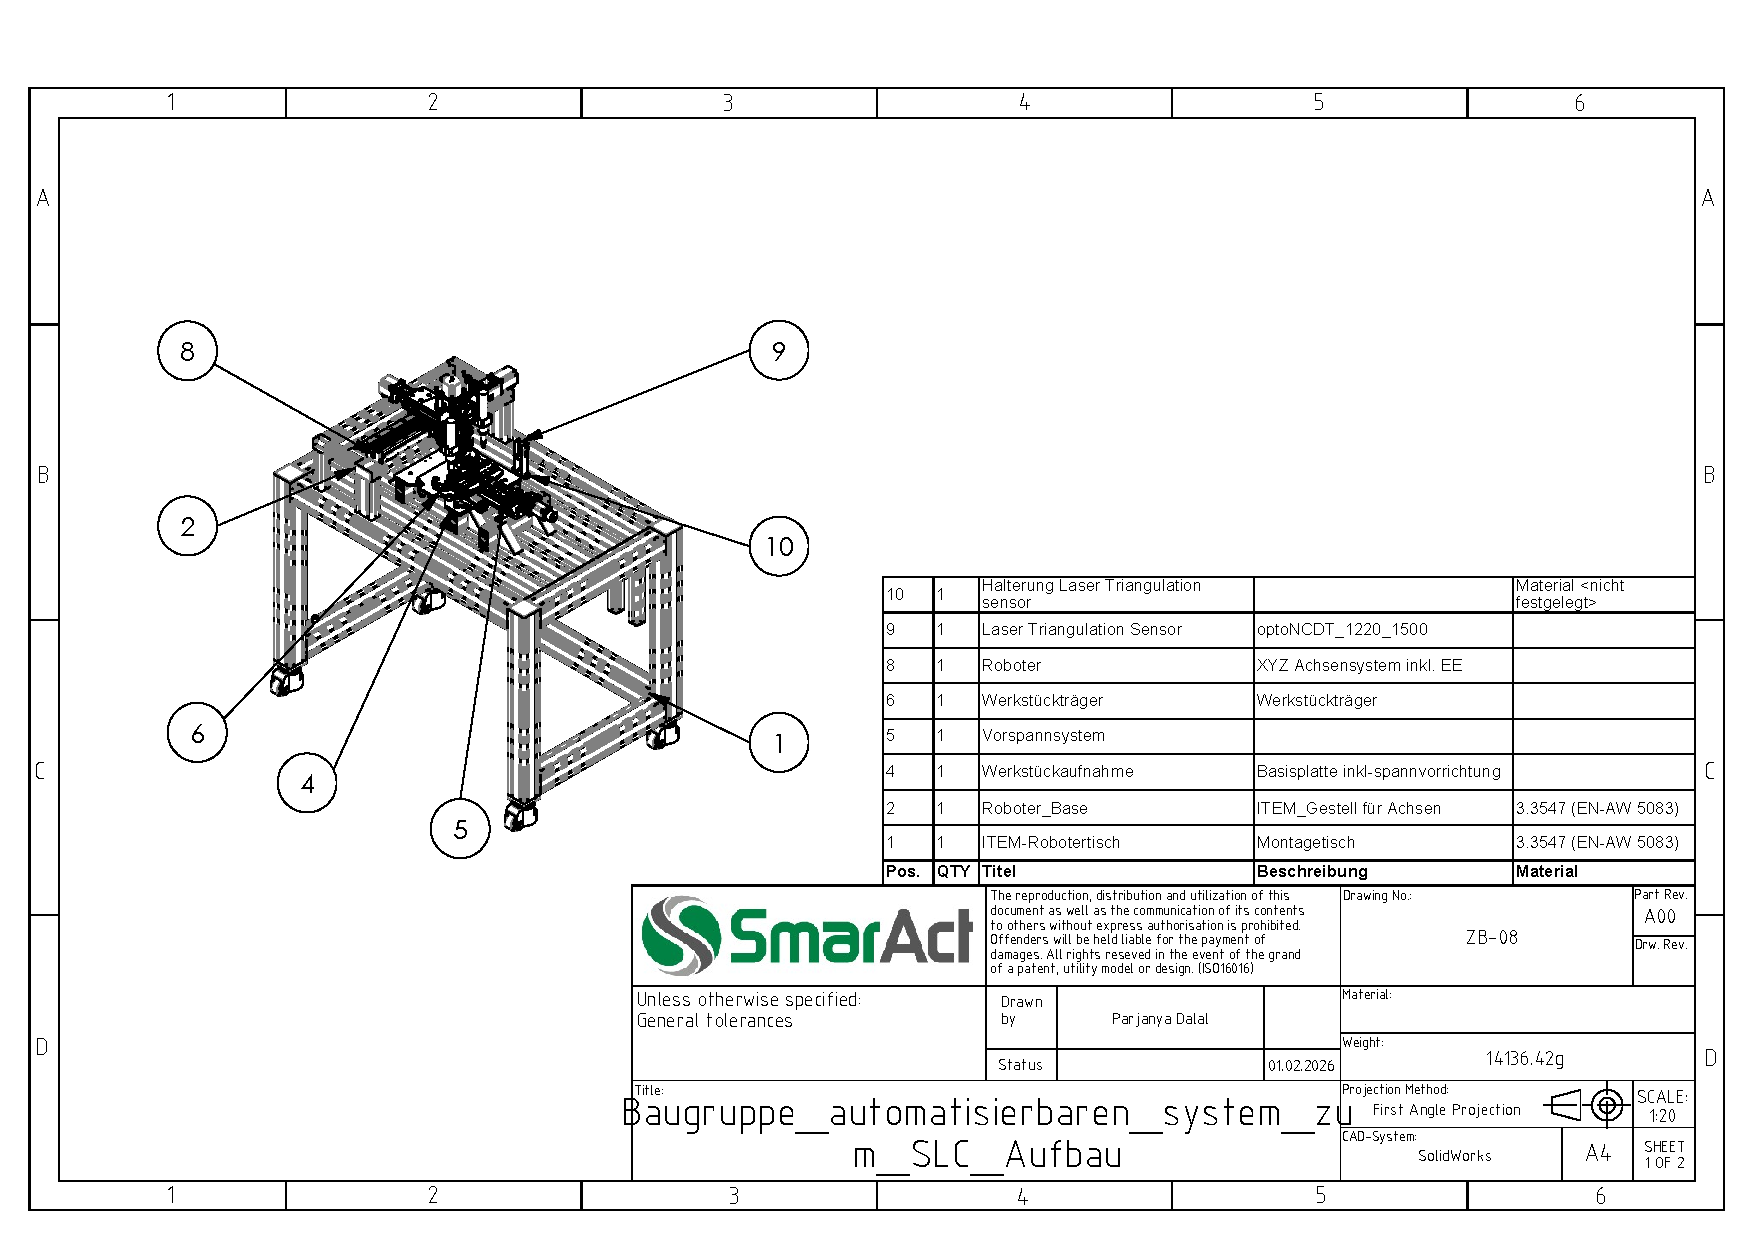
\includepdf[pages={-}, angle=90, scale=0.9]{Anhang/Gesamtbau_pdf.pdf}
\label{anhang:ee_2d}
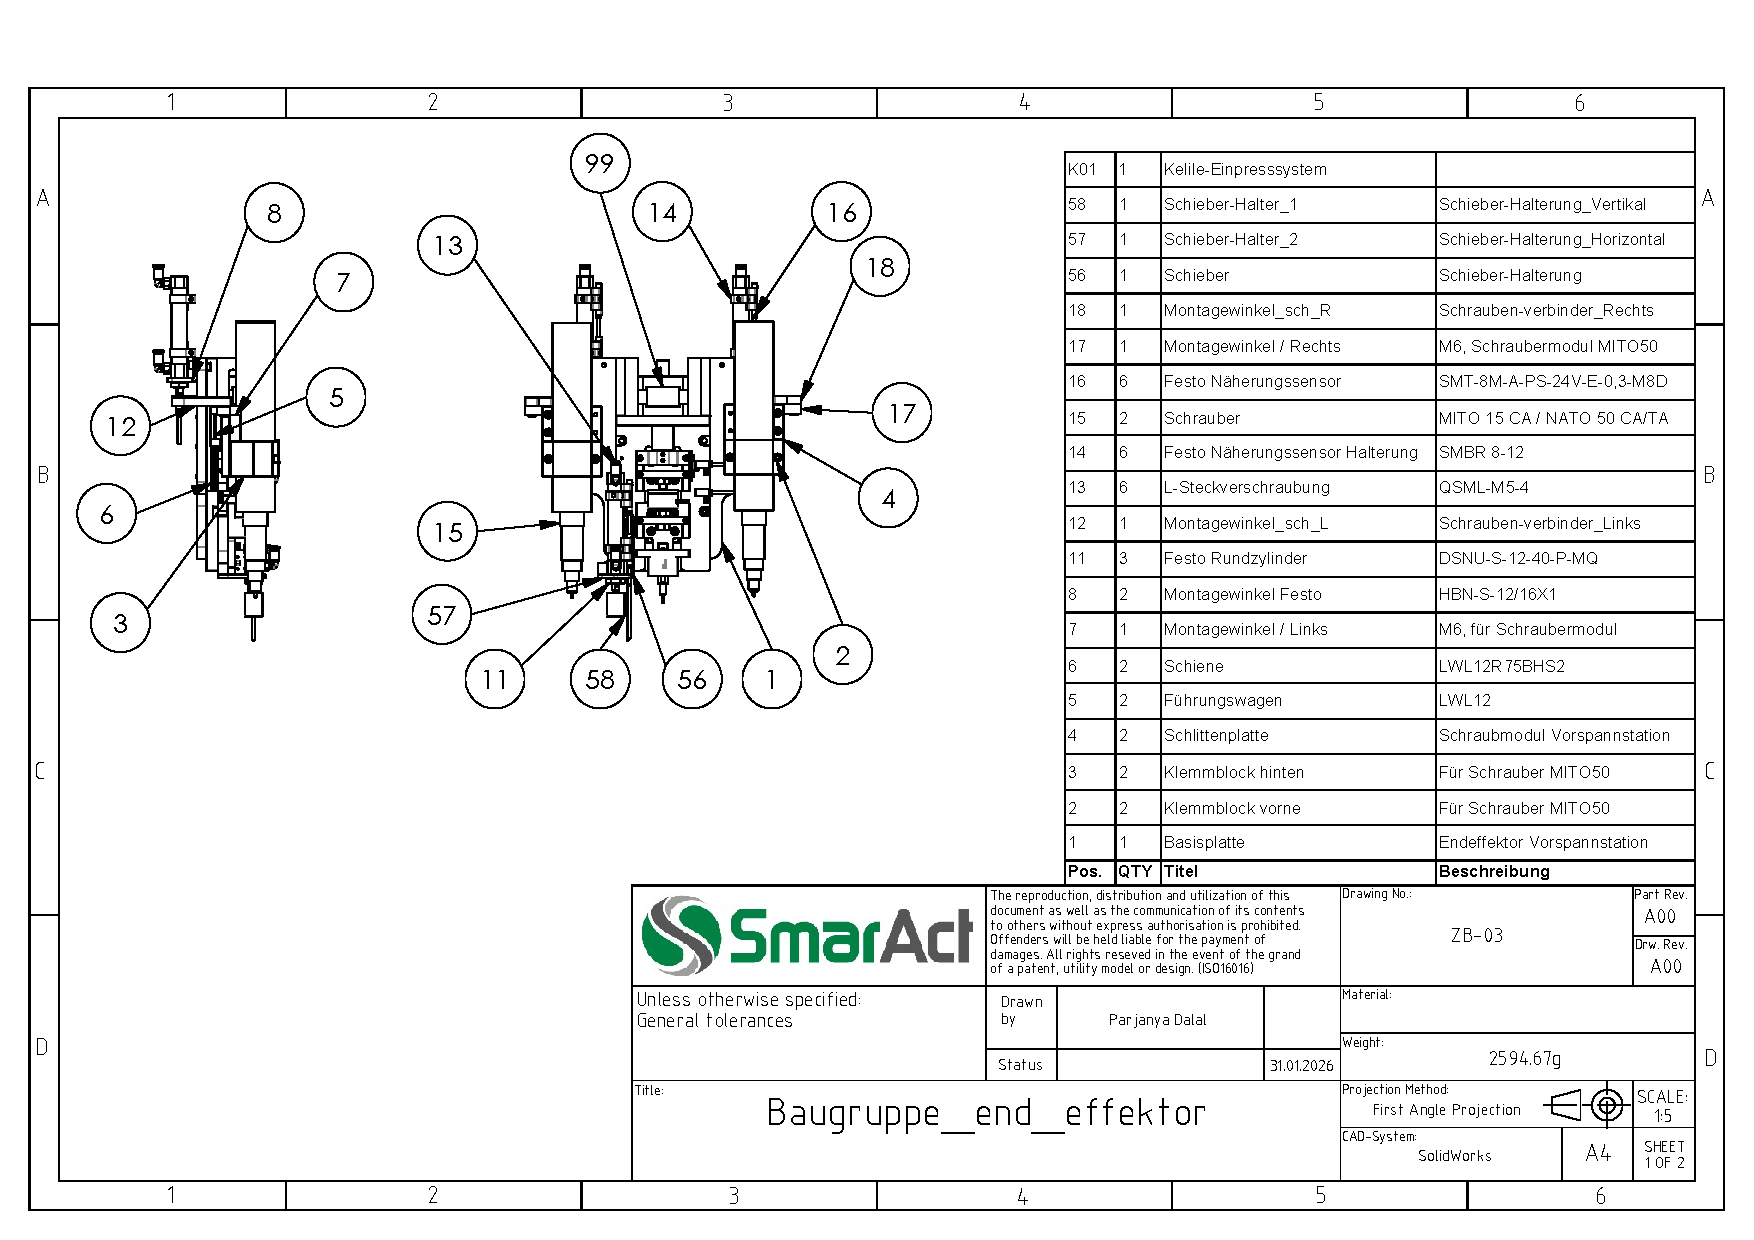
\includepdf[pages={-}, angle=90, scale=0.9]{Anhang/EE_pdf.pdf}
\label{anhang:achssystem}
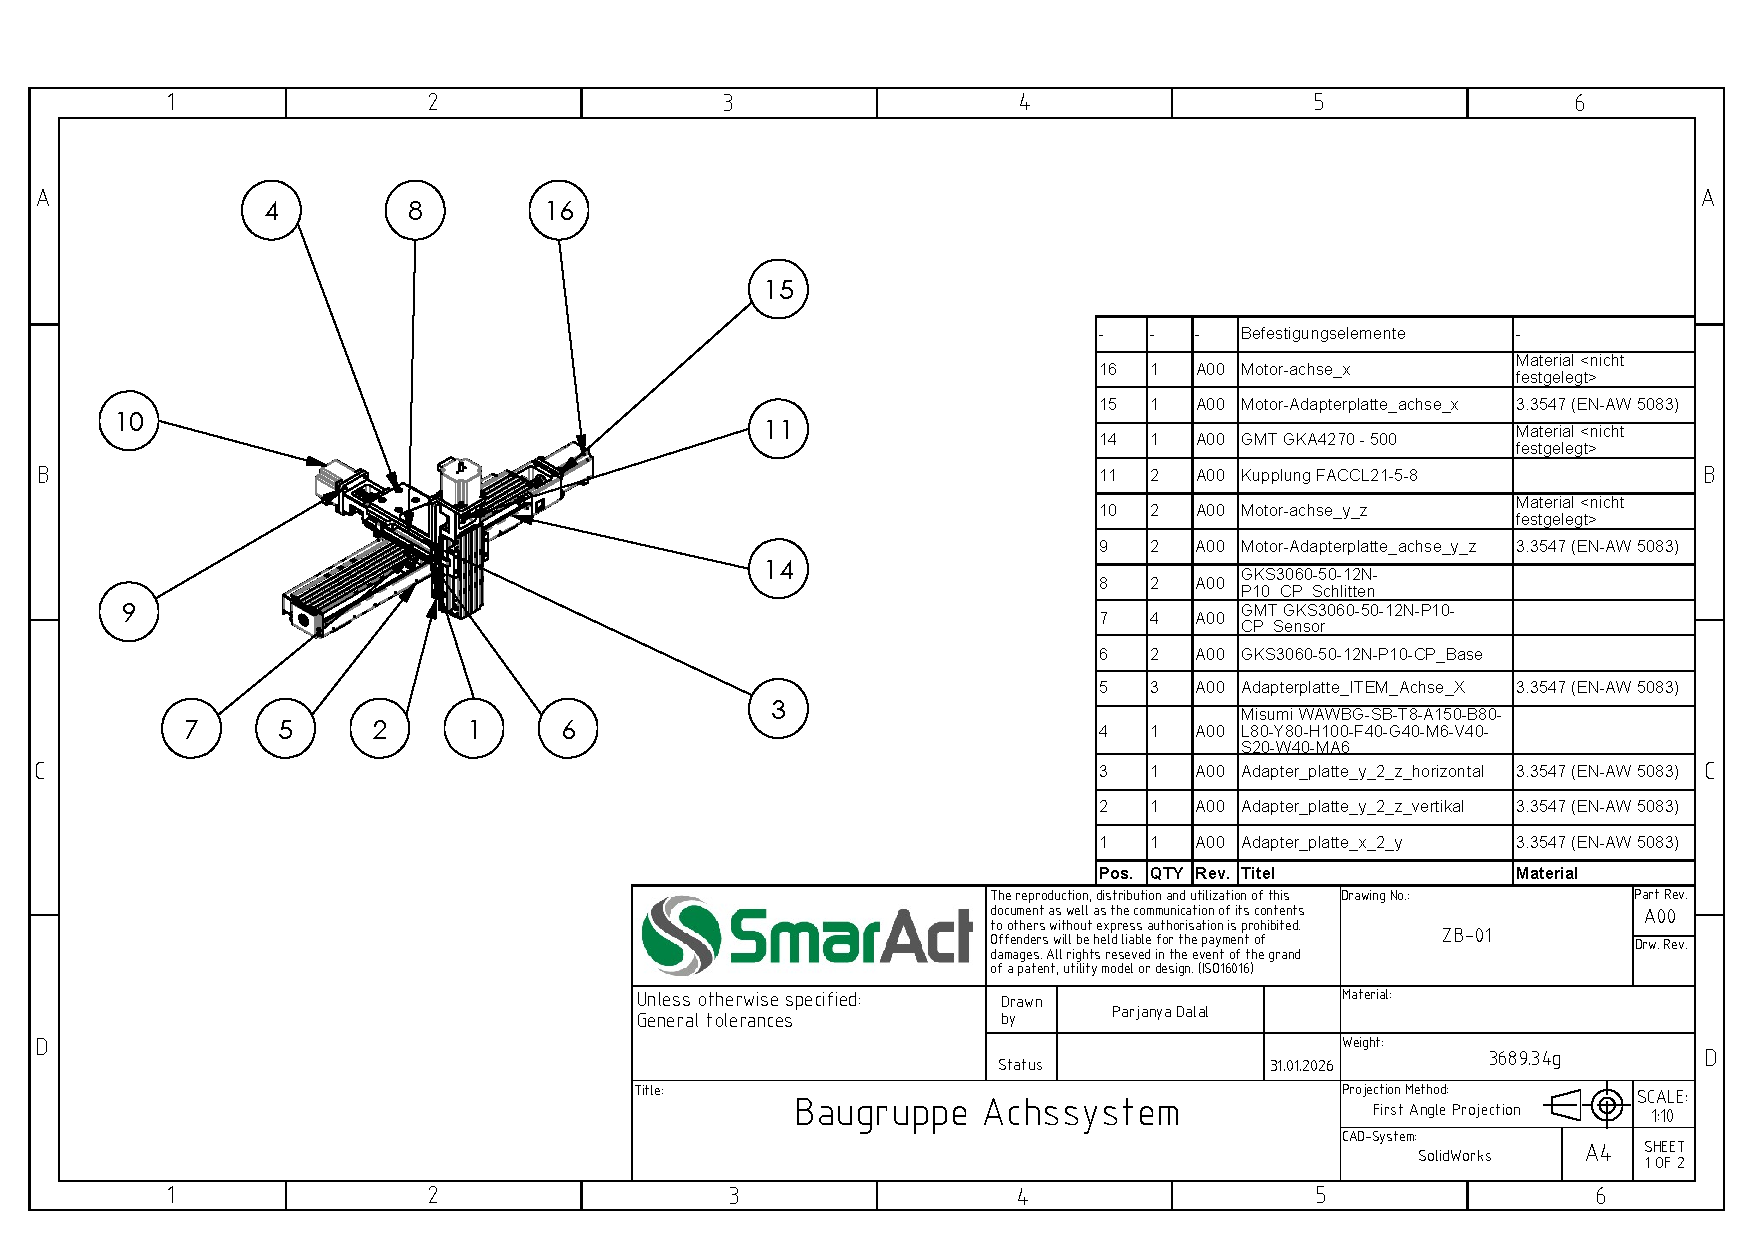
\includepdf[pages=-, angle=90 , scale=0.9]{Anhang/Achssystem_pdf.pdf}
\label{anhang:Werkst.}
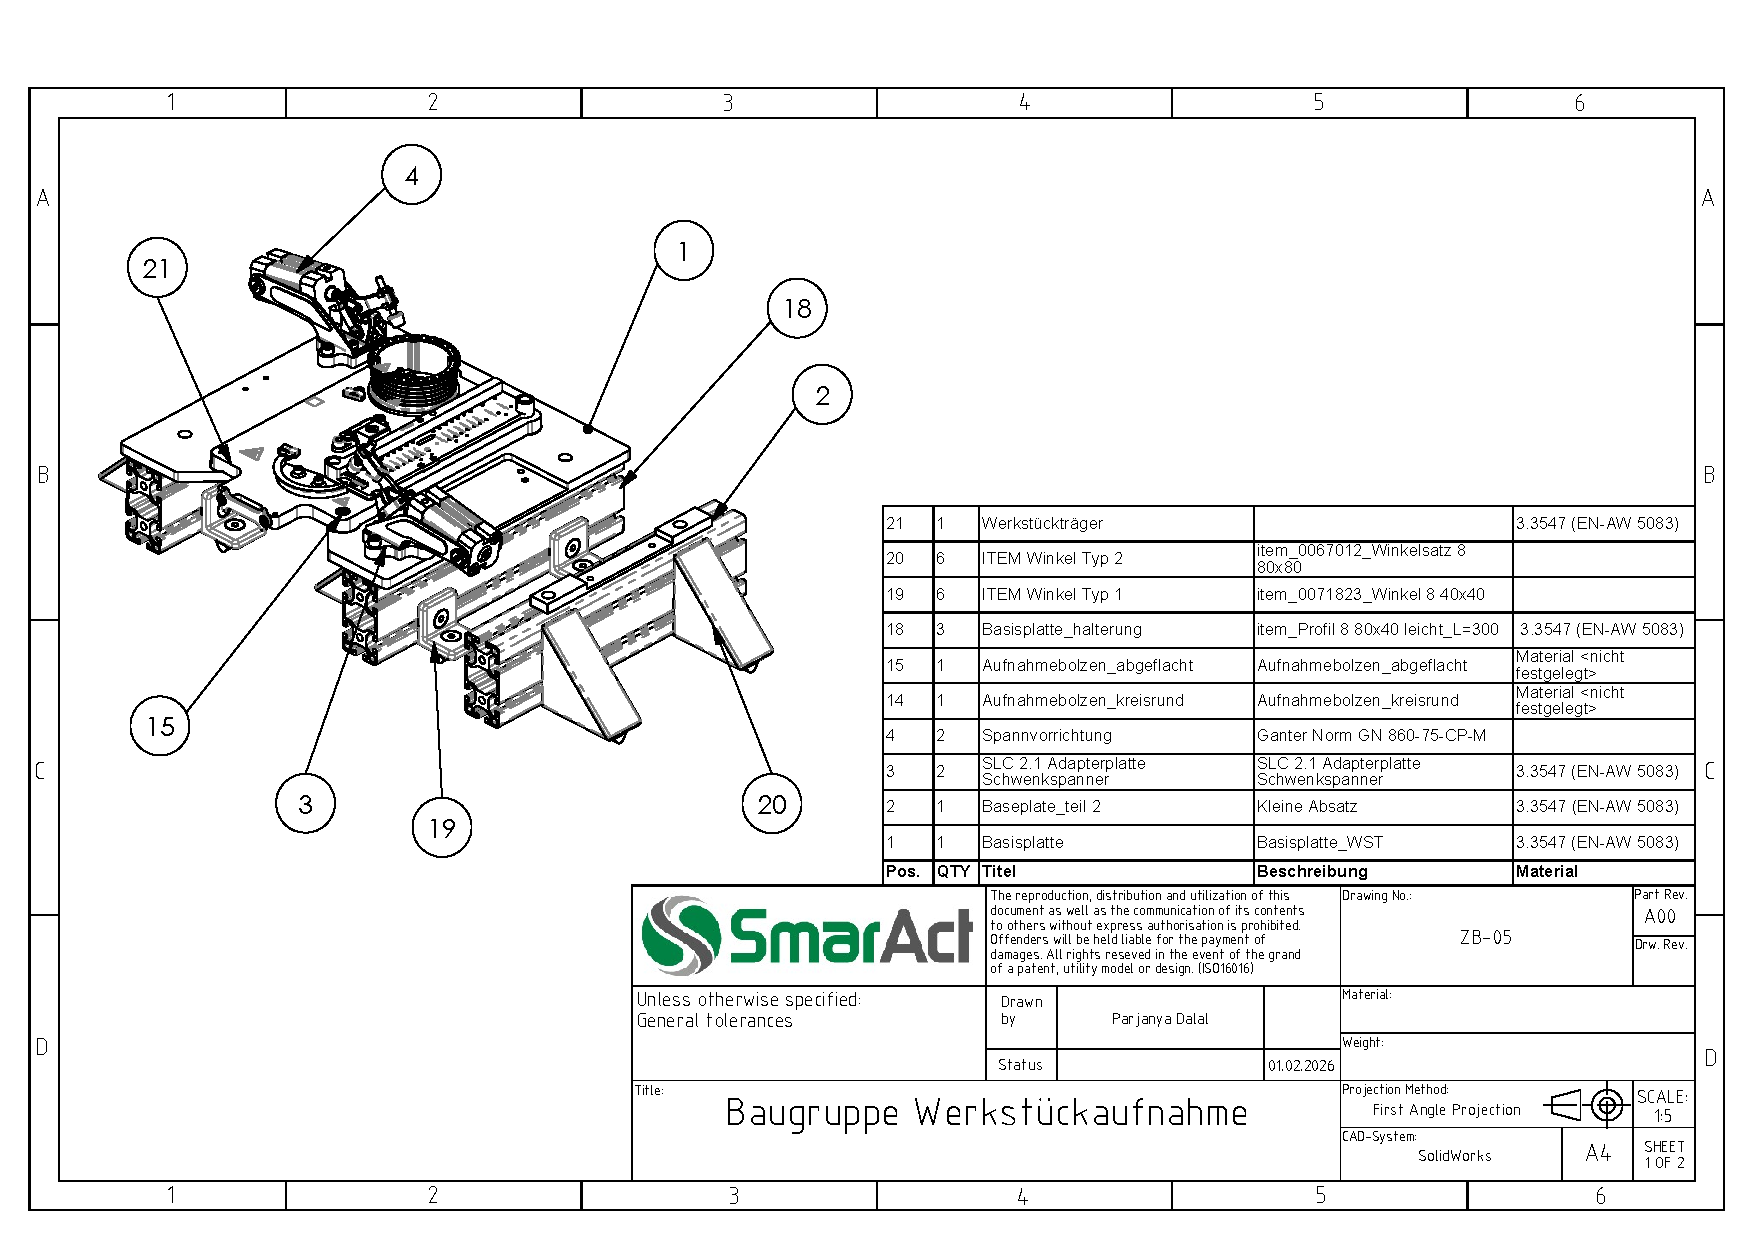
\includepdf[pages={-}, angle=90, scale=0.9]{Anhang/Werkst_pdf_1.pdf}
\end{landscape}
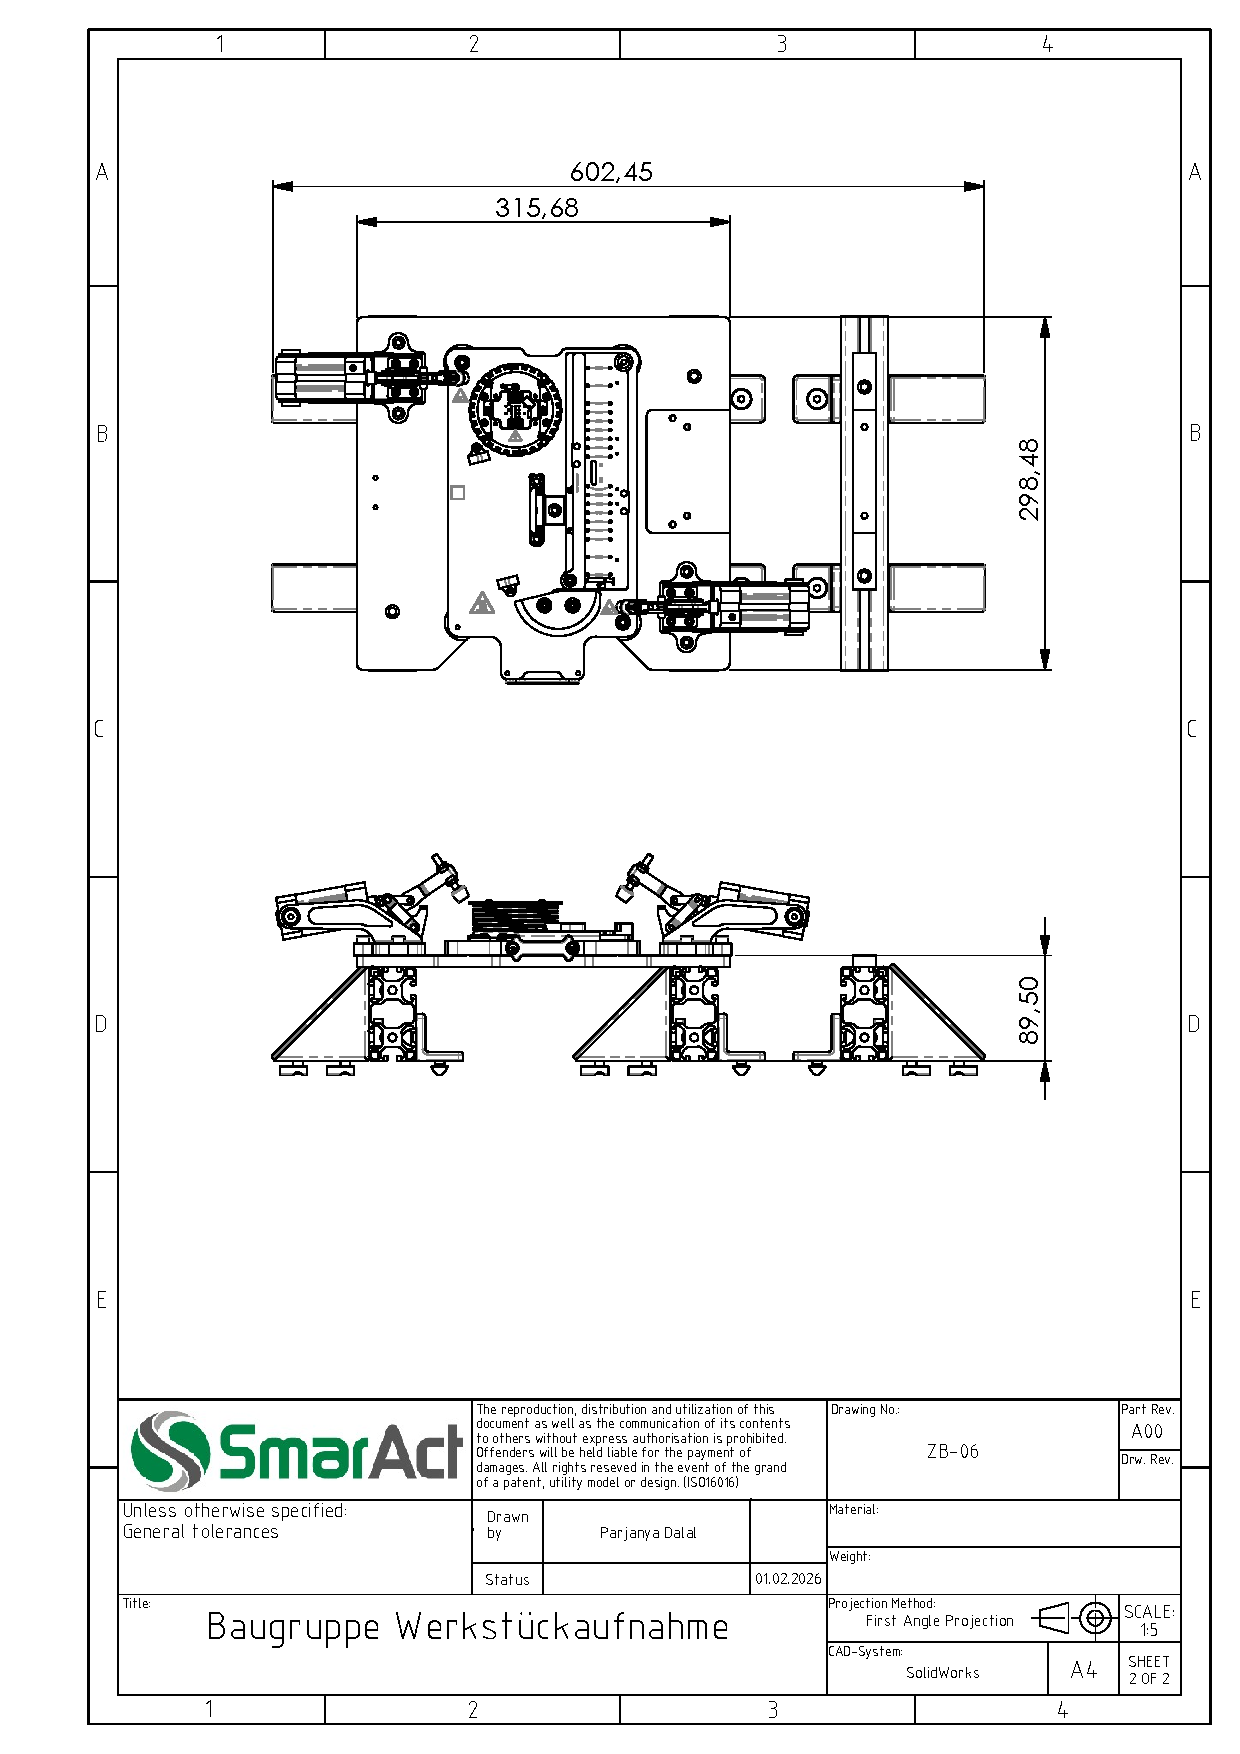
\includepdf[pages={-}, scale=0.9]{Anhang/Werkst_pdf_2.pdf}

\clearpage

\begin{landscape}
\section{Stückliste}
\subsection{Gesamt Stückliste}
{
\small
\setlength{\tabcolsep}{3pt}
\renewcommand{\arraystretch}{1.15}

\begin{longtable}{|l|l|l|l|l|p{4.6cm}|p{6.5cm}|}
\hline
\textbf{Nr.} & \textbf{Menge} & \textbf{Klassifikation} & \textbf{Kategorie} & \textbf{Benennung} & \textbf{Produkt / Typ} & \textbf{Erläuterung} \\
\hline
\endfirsthead

\hline
\textbf{Nr.} & \textbf{Menge} & \textbf{Klassifikation} & \textbf{Kategorie} & \textbf{Benennung} & \textbf{Produkt / Typ} & \textbf{Erläuterung} \\
\hline
\endhead

\endlastfoot

% ---------------- Base ----------------
B01 & 1 & COTS & Base & ITEM Roboter-Tisch & ITEM Profil 8 (Gestell) & Aluminiumprofil-Gestell mit Verbindern, Füßen und Tischplatte \\
\hline
B02 & 1 & COTS & Base & ITEM Roboter-Basis & ITEM Profil 8 (40×40, 40×80) & Aluminiumprofil-Gestell als Basisrahmen \\
\hline
B03 & 3 & COTS & Base & ITEM WST-Basis & ITEM Profil 8 (40×80) & Aluminiumprofil-Gestell zur Aufnahme der WST-Struktur \\
\hline
B04 & 1 & M & Base & WST-Basisplatte Teil 1 & Eigenfertigung (Aluminiumplatte) & Platte zur Aufnahme von WST und Vorspannstation \\
\hline
B05 & 1 & M & Base & WST-Basisplatte Teil 2 & Eigenfertigung (Aluminiumplatte) & Platte zur Aufnahme der Vorspannstation \\
\hline
B06 & 2 & COTS & Base & Passstifte & Passstifte & Fixierung des Werkstückträgers in definierter Position \\
\hline

% ---------------- Keileinpresssystem ----------------
K01 & 1 & M & Keileinpresssystem & Grundplatte & Eigenfertigung & Basisplatte des Keileinpresssystems \\
\hline
K02 & 1 & M & Keileinpresssystem & Motorhalterplatte & Eigenfertigung & Aufnahme des Vertikalantriebs \\
\hline
K03 & 2 & M & Keileinpresssystem & Motorhalter-Halterung & Eigenfertigung & Mechanische Fixierung der Motorhalterplatte \\
\hline
K04 & 1 & M & Keileinpresssystem & M4-Gewindeadapter & Eigenfertigung & Adapterelement zur Montage \\
\hline
K05 & 2 & COTS & Keileinpresssystem & Führungswagen & Misumi SSE2BLZ13G-100 & Linearführungswagen des Keileinpresssystems \\
\hline
K06 & 1 & M & Keileinpresssystem & Einpresskeil & Eigenfertigung & Keil zur Kraftübertragung auf das Führungspaket \\
\hline
K07 & 1 & M & Keileinpresssystem & Federstück & Eigenfertigung & Mechanisches Rückstellelement / Federaufnahme \\
\hline
K08 & 1 & COTS & Keileinpresssystem & Führungsschiene & Misumi SSE2BLZ13G-100 & Linearschiene des Keileinpresssystems \\
\hline
K09 & 1 & COTS & Keileinpresssystem & Kraftmessdose & KM26Z-50N & Kraftsensor zur Prozessüberwachung \\
\hline
K10 & 1 & COTS & Keileinpresssystem & DMS-Verstärker & ME GSV-1H 010/10kHz/2 & Signalaufbereitung der Kraftmessdose \\
\hline
K11 & 1 & COTS & Keileinpresssystem & Schrittmotor (vertikal) & Nanotec LGA421S14-B-UKAS-019 & Vertikalantrieb des Keileinpresssystems \\
\hline
K12 & 2 & COTS & Keileinpresssystem & Gabellichtschranke & Panasonic PM-F25 & Endlagenerfassung des Keilschlittens (2×) \\
\hline
K13 & 2 & COTS & Keileinpresssystem & Druckfeder & 6--10\,mm & Mechanische Vorspannung / Rückstellung \\
\hline
K14 & 1 & M & Keileinpresssystem & Lichtschranken-Pin & 3D-Druck & Betätigungselement für die Gabellichtschranken \\
\hline
K15 & 1 & M & Keileinpresssystem & Schlitten oben & Eigenfertigung & Bewegliches Führungselement (oberes Teil) \\
\hline
K16 & 1 & M & Keileinpresssystem & Schlitten unten & Eigenfertigung & Gegenstück des Schlittens (unteres Teil) \\
\hline
K17 & 1 & COTS & Keileinpresssystem & Universal-Gelenk & GDW1720-W & Mechanische Kraftübertragung / Ausgleich \\
\hline
K18 & 1 & M & Keileinpresssystem & Kraftsensorplatte unten & Eigenfertigung & Adapterplatte zur Integration der Kraftmessdose (unten) \\
\hline
K19 & 1 & M & Keileinpresssystem & Kraftsensorplatte oben & Eigenfertigung & Adapterplatte zur Integration der Kraftmessdose (oben) \\
\hline
K20 & 1 & M & Keileinpresssystem & Flansch & Eigenfertigung & Verbindungselement zum Antrieb / zur Struktur \\
\hline

% ---------------- Robotersystem ----------------
R01 & 1 & COTS & Robotersystem & Linearachse X & GKA4270-500-12N-P10 & Portalachse für horizontale Positionierung (X) \\
\hline
R02 & 1 & COTS & Robotersystem & Linearachse Y & GKS3060-50-12N-P5 & Querachse des Portals (Y) \\
\hline
R03 & 1 & COTS & Robotersystem & Linearachse Z & GKS3060-50-12N-P6 & Vertikalachse des Portals (Z) \\
\hline
R04 & 1 & COTS & Robotersystem & Schrittmotor X & Nanotec SCA5618L4204-B2 (NEMA 23, 3\,Nm) & Antrieb der X-Achse \\
\hline
R05 & 1 & COTS & Robotersystem & Schrittmotor Y & Nanotec SCB6018M4204-B (NEMA 23, 2\,Nm) & Antrieb der Y-Achse \\
\hline
R06 & 1 & COTS & Robotersystem & Schrittmotor Z & Nanotec SCB6018M4204-B (NEMA 23, 2\,Nm) & Antrieb der Z-Achse \\
\hline
R07 & 3 & M & Robotersystem & Adapterplatte ITEM–X & Eigenfertigung & Verbindung X-Achse mit ITEM-Gestell (3×) \\
\hline
R08 & 1 & M & Robotersystem & Adapterplatte X–Y & Eigenfertigung & Verbindung X- zu Y-Achse \\
\hline
R09 & 1 & M & Robotersystem & Adapterplatte Y–Z (1) & Eigenfertigung & Verbindung Y-Achse mit Zwischenplatte \\
\hline
R10 & 1 & M & Robotersystem & Adapterplatte Y–Z (2) & Eigenfertigung & Verbindung Zwischenplatte mit Z-Achse \\
\hline
R11 & 1 & COTS & Robotersystem & Winkelplatte & Misumi (90°-Befestigung) & Montageelement zur 90°-Befestigung \\
\hline

% ---------------- Schraubereinheit ----------------
S01 & 1 & M & Schraubereinheit & Endeffektor-Grundplatte & Eigenfertigung & Verbindung Adapterplatte Y--Z (2) mit Endeffektor \\
\hline
S02 & 2 & COTS & Schraubereinheit & Führungsschiene & LWL 12R75BHS2 & Linearschiene der Schraubereinheit (2×) \\
\hline
S03 & 2 & COTS & Schraubereinheit & Führungswagen & LWL 12 & Lineare Führung des Schraubschlittens (2×) \\
\hline
S04 & 2 & M & Schraubereinheit & Schlittenadapterplatte & Eigenfertigung & Verbindung Schlitten--Werkzeug (2×) \\
\hline
S05 & 2 & M & Schraubereinheit & Klemmblock hinten & Eigenfertigung & Fixierung des Schraubers (hinten, 2×) \\
\hline
S06 & 2 & M & Schraubereinheit & Klemmblock vorne & Eigenfertigung & Fixierung des Schraubers (vorne, 2×) \\
\hline
S07 & 2 & M & Schraubereinheit & Montagewinkel (Festo) & Eigenfertigung / Montagewinkel & Pneumatik-Anbindung der Schraubereinheit \\
\hline
S08 & 3 & COTS & Schraubereinheit & Pneumatikzylinder & Festo DSNU-S-12-40-P-MQ & Zustellbewegung der Schrauber \\
\hline
S09 & 6 & COTS & Schraubereinheit & L-Steckverschraubung & Festo L-Steckverschraubung & Pneumatische Verbindung (6×) \\
\hline
S10 & 6 & COTS & Schraubereinheit & Näherungssensor-Halter & Festo SMBR 8-12 & Halter für Näherungssensoren (6×) \\
\hline
S11 & 6 & COTS & Schraubereinheit & Näherungssensor & Festo SMT-8M-A-PS-24V-E-0,3-M8D & Endlagen-/Positionsabfrage (6×) \\
\hline
S12 & 1 & M & Schraubereinheit & Montagewinkel rechts & Eigenfertigung & Mechanische Verbindung (rechts) \\
\hline
S13 & 1 & M & Schraubereinheit & Montagewinkel links & Eigenfertigung & Mechanische Verbindung (links) \\
\hline
S14 & 1 & M & Schraubereinheit & Verbinder rechts & Eigenfertigung (L-Form) & Verbindung Piston--Schlitten (rechte Seite) \\
\hline
S15 & 1 & M & Schraubereinheit & Verbinder links & Eigenfertigung (L-Form) & Verbindung Piston--Schlitten (linke Seite) \\
\hline
S16 & 1 & COTS & Schraubereinheit & Schrauber SLC24 & MITO15CA & Automatischer Schrauber für SLC-24 \\
\hline
S17 & 1 & COTS & Schraubereinheit & Schrauber SLC17 & NATO50CA/TA & Automatischer Schrauber für SLC-17 \\
\hline

% ---------------- Schieber ----------------
SI01 & 1 & M & Schieber & Halterung vertikal & Eigenfertigung & Halterung Pneumatikzylinder vertikal \\
\hline
SI02 & 1 & M & Schieber & Halterung horizontal & Eigenfertigung & Halterung Pneumatikzylinder horizontal \\
\hline
SI03 & 1 & M & Schieber & Schieber & 3D-Druck & Provisorischer Schieber (3D-gedruckt) \\
\hline

% ---------------- Vorspannsystem ----------------
V01 & 1 & M & Vorspannsystem & Schraubstock & Eigenfertigung / Montage & Vorspannen der SLC-Führung (Einspannung) \\
\hline
V02 & 1 & COTS & Vorspannsystem & Kraftmessdose & KM26Z-500N & Messung der Vorspannkraft \\
\hline
V03 & 1 & COTS & Vorspannsystem & DMS-Verstärker & ME GSV-1H 010/10kHz/2 & Signalaufbereitung der Kraftmessdose \\
\hline
V04 & 1 & M & Vorspannsystem & Druckstange & Eigenfertigung & Verbindung Spindel--Kraftmessdose \\
\hline
V05 & 1 & M & Vorspannsystem & Adapterplatte unten & Eigenfertigung & Adapterplatte: Schlitten zur Schraubstockaufnahme \\
\hline
V06 & 1 & M & Vorspannsystem & Adapterplatte oben & Eigenfertigung & Adapterplatte: Schlitten zur Spindelmutter (Log Nut) \\
\hline
V07 & 2 & COTS & Vorspannsystem & Linearführungsschlitten & MISUMI SSE2BWZ16G-190 & Schlitten des Vorspannsystems (2×) \\
\hline
V08 & 1 & COTS & Vorspannsystem & Linearführungsschiene & NB Guide SERS15WA (Japan SM6722) & Schiene des Vorspannsystems \\
\hline
V09 & 1 & COTS & Vorspannsystem & Trapezgewindemutter & Tr12×3 Log Nut (im Gehäuse) & Spindelmutter im Gehäuse \\
\hline
V10 & 1 & COTS & Vorspannsystem & Trapezgewindespindel & Tr12×3 (gerollt, verlängert) & Linearantrieb der Vorspannmechanik \\
\hline
V11 & 1 & COTS & Vorspannsystem & Festlagergehäuse & dold FLB16-30/8 & Lagerung der Spindel / Adapter \\
\hline
V12 & 1 & COTS & Vorspannsystem & Schrittmotor & Nanotec ST4118D1804-B (NEMA 17, mit Bremse) & Antrieb der Vorspannspindel \\
\hline
V13 & 1 & COTS & Vorspannsystem & Kupplung & dold RB flexibel D18L25 (5{,}00/6{,}00\,mm) & Motor--Spindel-Verbindung \\
\hline
V14 & 1 & M & Vorspannsystem & Grundplatte & Eigenfertigung & Aufnahme / Halterung des Vorspannsystems \\
\hline

% ---------------- Steuerung ----------------
C01 & 1 & COTS & Steuerung & Motorcontroller & TMCM-6110 & Ansteuerung der Schrittmotorachsen \\
\hline
C02 & 4 & COTS & Steuerung & Magnetventil & Festo & Pneumatische Ansteuerung (z.\,B. Zylinder) \\
\hline
C03 & 1 & COTS & Steuerung & Laser-Triangulationssensor & optoNCDT 1220-500 & Positionsmessung des Schlittens \\
\hline
C04 & 1 & COTS & Steuerung & Modbus-Koppler & WAGO 750-362 & Feldbus-Anbindung \\
\hline
C05 & 1 & COTS & Steuerung & Potentialeinspeisung & WAGO 750-602 & 24-VDC-Versorgung / Einspeisung \\
\hline
C06 & 1 & COTS & Steuerung & Digitalausgangsmodul & WAGO 750-531 & Aktoransteuerung (DO) \\
\hline
C07 & 2 & COTS & Steuerung & Analogeingangsmodul & WAGO 750-466 & Sensoranbindung (AI) \\
\hline
C08 & 1 & COTS & Steuerung & Endmodul & WAGO 750-600 & Abschluss der WAGO-Klemme \\
\hline
C09 & 1 & COTS & Steuerung & Netzteil & Phoenix Contact UNO-PS/1AC/24DC/60W & 24-VDC-Stromversorgung \\
\hline
C10 & 6 & COTS & Steuerung & Koppelrelais & Finder 34.51.7.024.0050 & Galvanische Trennung / Relaiskopplung (6×) \\
\hline

\caption{Gesamtstückliste des automatisierten Montagesystems}
\label{tab:gesamt_stueckliste}
\end{longtable}
}
\end{landscape}

\clearpage

\section{Berechnungen}
\label{anhang:berechnungen}
%======================================================================
\subsection{Achssysteme X-, Y- und Z-Achse (eigene Auslegung)}
%======================================================================

\subsubsection{Berechnung der theoretischen Schrittauflösung}

Für alle drei Achsen kommen Schrittmotoren mit einem Schrittwinkel von \SI{1,8}{\degree} zum Einsatz.
Daraus ergeben sich
\begin{equation}
N_\text{Vollschritte}=\frac{360^\circ}{1,8^\circ}=200\ \text{Vollschritte/U}.
\end{equation}

Die Microstep-Auflösung ist über den Achsparameter SAP~140 aus der Trinamic Steuerung eingestellt. In der verwendeten Konfiguration gilt:
\begin{align}
\text{Achse 0 (X):} \quad & \text{SAP 140} = 5 \Rightarrow m_X = 32\ \text{Microsteps/Vollschritt} \\
\text{Achse 1 (Y):} \quad & \text{SAP 140} = 4 \Rightarrow m_Y = 16\ \text{Microsteps/Vollschritt} \\
\text{Achse 2 (Z):} \quad & \text{SAP 140} = 4 \Rightarrow m_Z = 16\ \text{Microsteps/Vollschritt}
\end{align}

Damit ergeben sich die Microsteps pro Umdrehung:
\begin{align}
N_{\mu\text{steps/U},X} &= 200\cdot 32 = 6400,\\
N_{\mu\text{steps/U},Y} &= 200\cdot 16 = 3200,\\
N_{\mu\text{steps/U},Z} &= 200\cdot 16 = 3200.
\end{align}

Die Spindelsteigungen ergeben sich aus den verwendeten Achstypen:
\begin{align}
\text{X-Achse:} \quad & \text{GKA4270-500-12N-P10} \Rightarrow p_X=\SI{10}{mm/U}
 \\
\text{Y-/Z-Achse:} \quad & \text{GKS3060-50-12N-P5} \Rightarrow p_Y=p_Z=\SI{5}{mm/U}
\end{align}
Eine Übersetzung ist nicht vorhanden ($1{:}1$).

Die lineare Schrittauflösung lautet:
\begin{equation}
s_{\mu\text{step}}=\frac{p}{N_{\mu\text{steps/U}}}.
\end{equation}

\paragraph{X-Achse:}
\begin{equation}
s_{\mu\text{step},X}=\frac{10}{6400}
=\SI{0,0015625}{mm}
=\SI{1,56}{\micro m}.
\end{equation}

\paragraph{Y- und Z-Achse:}
\begin{equation}
s_{\mu\text{step},Y/Z}=\frac{5}{3200}
=\SI{0,0015625}{mm}
=\SI{1,56}{\micro m}.
\end{equation}

Die geforderte Positionsauflösung von $\leq \SI{15}{\micro m}$ wird somit auf allen Achsen deutlich unterschritten.
Es ist zu beachten, dass es sich hierbei um eine theoretische Schrittauflösung handelt; mechanische Einflüsse
(z.\,B. Spindelsteigungsfehler, Nachgiebigkeiten, Reibung und Spiel) sind hierin nicht enthalten.

%----------------------------------------------------------------------
\subsubsection{Berechnung der minimal erforderlichen Microstepping-Auflösung}
%----------------------------------------------------------------------

Für die geforderte maximale Schrittweite $s_\text{max}=\SI{15}{\micro m}=\SI{0,015}{mm}$ gilt:
\begin{equation}
\frac{p}{200\cdot m}\leq 0,015.
\end{equation}

\paragraph{X-Achse ($p=\SI{10}{mm}$):}
\begin{equation}
m \geq \frac{10}{200\cdot 0,015} = 3,33
\Rightarrow m_\text{min}=4.
\end{equation}

\paragraph{Y- und Z-Achse ($p=\SI{5}{mm}$):}
\begin{equation}
m \geq \frac{5}{200\cdot 0,015} = 1,67
\Rightarrow m_\text{min}=2.
\end{equation}

Die eingestellten Microstepping-Stufen ($m_X=32$, $m_{Y/Z}=16$) bieten somit eine ausreichende Reserve.

%----------------------------------------------------------------------
\subsubsection{Umrechnung der TMCL-Geschwindigkeitsparameter}
%----------------------------------------------------------------------

Die maximale Positioniergeschwindigkeit ist in der Steuerung über SAP~4 eingestellt:
\begin{align}
\text{SAP 4, Achse 0 (X)} &= 2000,\\
\text{SAP 4, Achse 1 (Y)} &= 2000,\\
\text{SAP 4, Achse 2 (Z)} &= 2000.
\end{align}

Zusätzlich ist der Pulse Divider über SAP~154 gesetzt:
\begin{equation}
\text{pulse\_div}=\text{SAP 154}=5 \quad \text{(für alle Achsen)}.
\end{equation}

Gemäß der TMCL-Parametrierlogik wird aus dem internen Geschwindigkeitswert eine Schrittfrequenz
(pps, pulses per second) bestimmt. Für die vorliegende Konfiguration ergibt sich:
\begin{equation}
v_\text{pps}\approx \SI{15259}{pps}.
\end{equation}

Zur Umrechnung in eine lineare Geschwindigkeit wird die Schrittzahl pro Millimeter benötigt:
\begin{equation}
\mu\text{steps/mm}=\frac{200\cdot m}{p}.
\end{equation}

\paragraph{X-Achse:}
\begin{equation}
\mu\text{steps/mm}_X=\frac{200\cdot 32}{10} = 640.
\end{equation}

\paragraph{Y- und Z-Achse:}
\begin{equation}
\mu\text{steps/mm}_{Y/Z}=\frac{200\cdot 16}{5} = 640.
\end{equation}

Damit ergibt sich (hier identisch für alle Achsen) die maximale lineare Geschwindigkeit:
\begin{equation}
v_{\max}=\frac{v_\text{pps}}{\mu\text{steps/mm}}
=\frac{15259}{640}
\approx \SI{23,84}{mm/s}.
\end{equation}

%----------------------------------------------------------------------
\subsubsection{Umrechnung der TMCL-Beschleunigungsparameter}
%----------------------------------------------------------------------

Die maximale Beschleunigung ist in der Steuerung über SAP~5 eingestellt:
\begin{align}
\text{SAP 5, Achse 0 (X)} &= 1000,\\
\text{SAP 5, Achse 1 (Y)} &= 1000,\\
\text{SAP 5, Achse 2 (Z)} &= 1000.
\end{align}

Zusätzlich sind Ramp Divider und Pulse Divider gesetzt:
\begin{equation}
\text{ramp\_div}=\text{SAP 153}=5,\qquad
\text{pulse\_div}=\text{SAP 154}=5
\quad \text{(für alle Achsen)}.
\end{equation}

Für die vorliegende Konfiguration ergibt sich eine Schritt-Beschleunigung von:
\begin{equation}
a_\text{pps} \approx \SI{1,164e5}{pps^2}.
\end{equation}

Die lineare Beschleunigung folgt zu:
\begin{equation}
a_{\max}=\frac{a_\text{pps}}{\mu\text{steps/mm}}
=\frac{1,164\cdot 10^5}{640}
\approx \SI{182}{mm/s^2}
=\SI{0,182}{m/s^2}.
\end{equation}

%----------------------------------------------------------------------
\subsubsection{Berechnung der idealisierten Fahrzeiten}
%----------------------------------------------------------------------

Zur Plausibilitätsprüfung werden idealisierte Fahrzeiten ohne Berücksichtigung von Rampenanteilen berechnet:
\begin{equation}
t \approx \frac{s}{v_{\max}}.
\end{equation}

\paragraph{X-Achse (max. Verfahrweg $s=\SI{413}{mm}$):}
\begin{equation}
t_X \approx \frac{413}{23,84}\approx \SI{17,3}{s}.
\end{equation}

\paragraph{Y- und Z-Achse (Hub $s=\SI{50}{mm}$):}
\begin{equation}
t_{Y/Z} \approx \frac{50}{23,84}\approx \SI{2,10}{s}.
\end{equation}

Die berechneten Zeiten dienen ausschließlich als Plausibilitätsprüfung; in der realen Bewegung erhöhen sich die
Fahrzeiten durch Beschleunigungs- und Verzögerungsphasen.

%======================================================================
\subsection{Motorauswahl und Nachweis gegen Schrittverlust}
%======================================================================

\subsubsection{Eingangsgrößen aus Datenblättern und Annahmen}

Für die verwendeten Schrittmotoren werden die Haltemomente aus den Datenblättern verwendet:

\begin{align}
M_{H,\text{SCA}} &= \SI{230}{Ncm} = \SI{2,30}{Nm},\\
M_{H,\text{SCB}} &= \SI{200}{Ncm} = \SI{2,00}{Nm}.
\end{align}

\noindent
Dabei kommen folgende Schrittmotoren zum Einsatz:
\begin{itemize}
  \item Nanotec SCA5618L4204-B2 \cite{nanotec_sca5618}
  \item Nanotec SCB6018M4204-B \cite{nanotec_scb6018}
\end{itemize}


Da im Herstellerdatenblatt der Linearachsen keine Angaben zur Reibkraft und zum Wirkungsgrad des Spindeltriebs
vorliegen, werden konservative Annahmen getroffen:
\begin{align}
F_{\text{reib},X} &= F_{\text{reib},Y} = F_{\text{reib},Z} = \SI{10}{N},\\
\eta &= 0{,}9 \qquad \text{(Annahme für Kugelgewindetrieb)}.
\end{align}

\paragraph{Hinweis zur Z-Achse (Kugelgewindetrieb, Haltestrom):}
Die Z-Achse basiert auf einem Kugelgewindetrieb (ball screw drive). Eine geometrische Selbsthemmung ist hierbei
nicht gegeben. In praktischen Tests wurde bei stromloser Achse kein Absinken beobachtet; dies ist auf detentes
Motormoment sowie Reib- und Verlustanteile im System zurückzuführen, stellt jedoch keinen garantierten
Sicherheitsmechanismus dar. Daher wird die Z-Achse im Stillstand mit Haltestrom betrieben.

%----------------------------------------------------------------------
\subsubsection{Berechnung der Motordrehzahl}
%----------------------------------------------------------------------

Die erforderliche Motordrehzahl ergibt sich aus der maximalen linearen Achsgeschwindigkeit und der Spindelsteigung
(Übersetzung $1{:}1$):
\begin{equation}
n_\text{rpm}=60\cdot \frac{v_{\max}}{p}.
\end{equation}

\paragraph{X-Achse ($p=\SI{10}{mm}$):}
\begin{equation}
n_{\text{rpm},X}=60\cdot \frac{23,84}{10}\approx \SI{143}{rpm}.
\end{equation}

\paragraph{Y- und Z-Achse ($p=\SI{5}{mm}$):}
\begin{equation}
n_{\text{rpm},Y/Z}=60\cdot \frac{23,84}{5}\approx \SI{286}{rpm}.
\end{equation}

%----------------------------------------------------------------------
\subsubsection{Berechnung der erforderlichen Linearkraft}
%----------------------------------------------------------------------

Die resultierende Linearkraft wird als Summe aus Trägheits-, Reibungs- und (für die Z-Achse) Gewichtskraftanteil
angesetzt:
\begin{equation}
F_\text{soll}=F_\text{träg}+F_\text{reib}+F_g.
\end{equation}

Der Trägheitsanteil lautet:
\begin{equation}
F_\text{träg}=m\cdot a_{\max}.
\end{equation}

Die bewegten Massen wurden aus der Konstruktion abgeleitet:
\begin{align}
m_X&=\SI{7,92}{kg},&
m_Y&=\SI{6,33}{kg},&
m_Z&=\SI{3,25}{kg}.
\end{align}

Mit $a_{\max}=\SI{0,182}{m/s^2}$ ergeben sich die Trägheitskräfte:
\begin{align}
F_{\text{träg},X}&=7,92\cdot 0,182 \approx \SI{1,441}{N},\\
F_{\text{träg},Y}&=6,33\cdot 0,182 \approx \SI{1,152}{N},\\
F_{\text{träg},Z}&=3,25\cdot 0,182 \approx \SI{0,592}{N}.
\end{align}

Für die Z-Achse (Bewegung nach oben) wird zusätzlich die Gewichtskraft berücksichtigt:
\begin{equation}
F_{g,Z}=m_Z\cdot g=3,25\cdot 9,81 \approx \SI{31,88}{N}.
\end{equation}

Damit ergeben sich die erforderlichen Kräfte (mit $F_{\text{reib}}=\SI{10}{N}$):
\begin{align}
F_{\text{soll},X} &\approx 1,441 + 10 = \SI{11,441}{N},\\
F_{\text{soll},Y} &\approx 1,152 + 10 = \SI{11,152}{N},\\
F_{\text{soll},Z,\uparrow} &\approx 0,592 + 10 + 31,88 = \SI{42,472}{N}.
\end{align}

%----------------------------------------------------------------------
\subsubsection{Berechnung des erforderlichen Spindelmoments}
%----------------------------------------------------------------------

Die Umrechnung der linearen Kraft in ein erforderliches Spindelmoment erfolgt über:
\begin{equation}
M_\text{soll}=\frac{F_\text{soll}\cdot p}{2\pi \cdot \eta}.
\end{equation}

Mit $p_X=\SI{10}{mm}=\SI{0,01}{m}$, sowie $p_{Y}=p_{Z}=\SI{5}{mm}=\SI{0,005}{m}$ und $\eta=0,9$ ergibt sich:
\begin{align}
M_{\text{soll},X} &\approx \frac{11,441\cdot 0,01}{2\pi\cdot 0,9} \approx \SI{0,02023}{Nm}=\SI{20,2}{Nmm},\\
M_{\text{soll},Y} &\approx \frac{11,152\cdot 0,005}{2\pi\cdot 0,9} \approx \SI{0,00986}{Nm}=\SI{9,86}{Nmm},\\
M_{\text{soll},Z,\uparrow} &\approx \frac{42,472\cdot 0,005}{2\pi\cdot 0,9} \approx \SI{0,03755}{Nm}=\SI{37,6}{Nmm}.
\end{align}

%----------------------------------------------------------------------
\subsubsection{Sicherheitsnachweis gegen Schrittverlust}
%----------------------------------------------------------------------

Schrittverlust wird vermieden, wenn das verfügbare Pull-out-Moment des Motors bei der jeweiligen Betriebsdrehzahl größer ist als das erforderliche Moment. Der Sicherheitsfaktor wird definiert als:
\begin{equation}
S=\frac{M_\text{ist}(n)}{M_\text{soll}}.
\end{equation}
Es muss gelten:
\begin{equation}
S>1.
\end{equation}

Für eine konservative Abschätzung wird das verfügbare Moment im relevanten Drehzahlbereich mit \num{50}\,\% des Haltemoments angesetzt (sicherheitsseitige Näherung bei fehlender exakter Auswertung der Kennlinie):
\begin{align}
M_{\text{ist},X} &= 0,5\cdot M_{H,\text{SCA}} = 0,5\cdot \SI{2,30}{Nm}=\SI{1,15}{Nm},\\
M_{\text{ist},Y/Z} &= 0,5\cdot M_{H,\text{SCB}} = 0,5\cdot \SI{2,00}{Nm}=\SI{1,00}{Nm}.
\end{align}

Damit ergeben sich die Sicherheitsfaktoren:
\begin{align}
S_X &\approx \frac{1,15}{0,02023} \approx 56,8,\\
S_Y &\approx \frac{1,00}{0,00986} \approx 101,4,\\
S_Z &\approx \frac{1,00}{0,03755} \approx 26,6.
\end{align}

\begin{table}[H]
\centering
\small
\setlength{\tabcolsep}{5pt}
\renewcommand{\arraystretch}{1.2}
\begin{tabular}{|l|c|c|c|c|}
\hline
\textbf{Achse} & $p$ [mm] & $M_\text{soll}$ [Nmm] & $M_\text{ist}$ [Nmm] & $S$ \\
\hline
X (SCA5618L4204-B2) & 10 & 20,2 & 1150 & 56,8 \\
\hline
Y (SCB6018M4204-B)  & 5  & 9,86 & 1000 & 101,4 \\
\hline
Z (SCB6018M4204-B)  & 5  & 37,6 & 1000 & 26,6 \\
\hline
\end{tabular}
\caption{Konservativer Nachweis gegen Schrittverlust durch Vergleich von erforderlichem und verfügbarem Motormoment.}
\label{tab:schrittverlust_nachweis}
\end{table}

\clearpage

\section{Schaltplan}
\label{anhang:schaltplan}
\subsection{TMCM-6110 Motor Steuerung}
\begin{figure}[H]
    \centering
    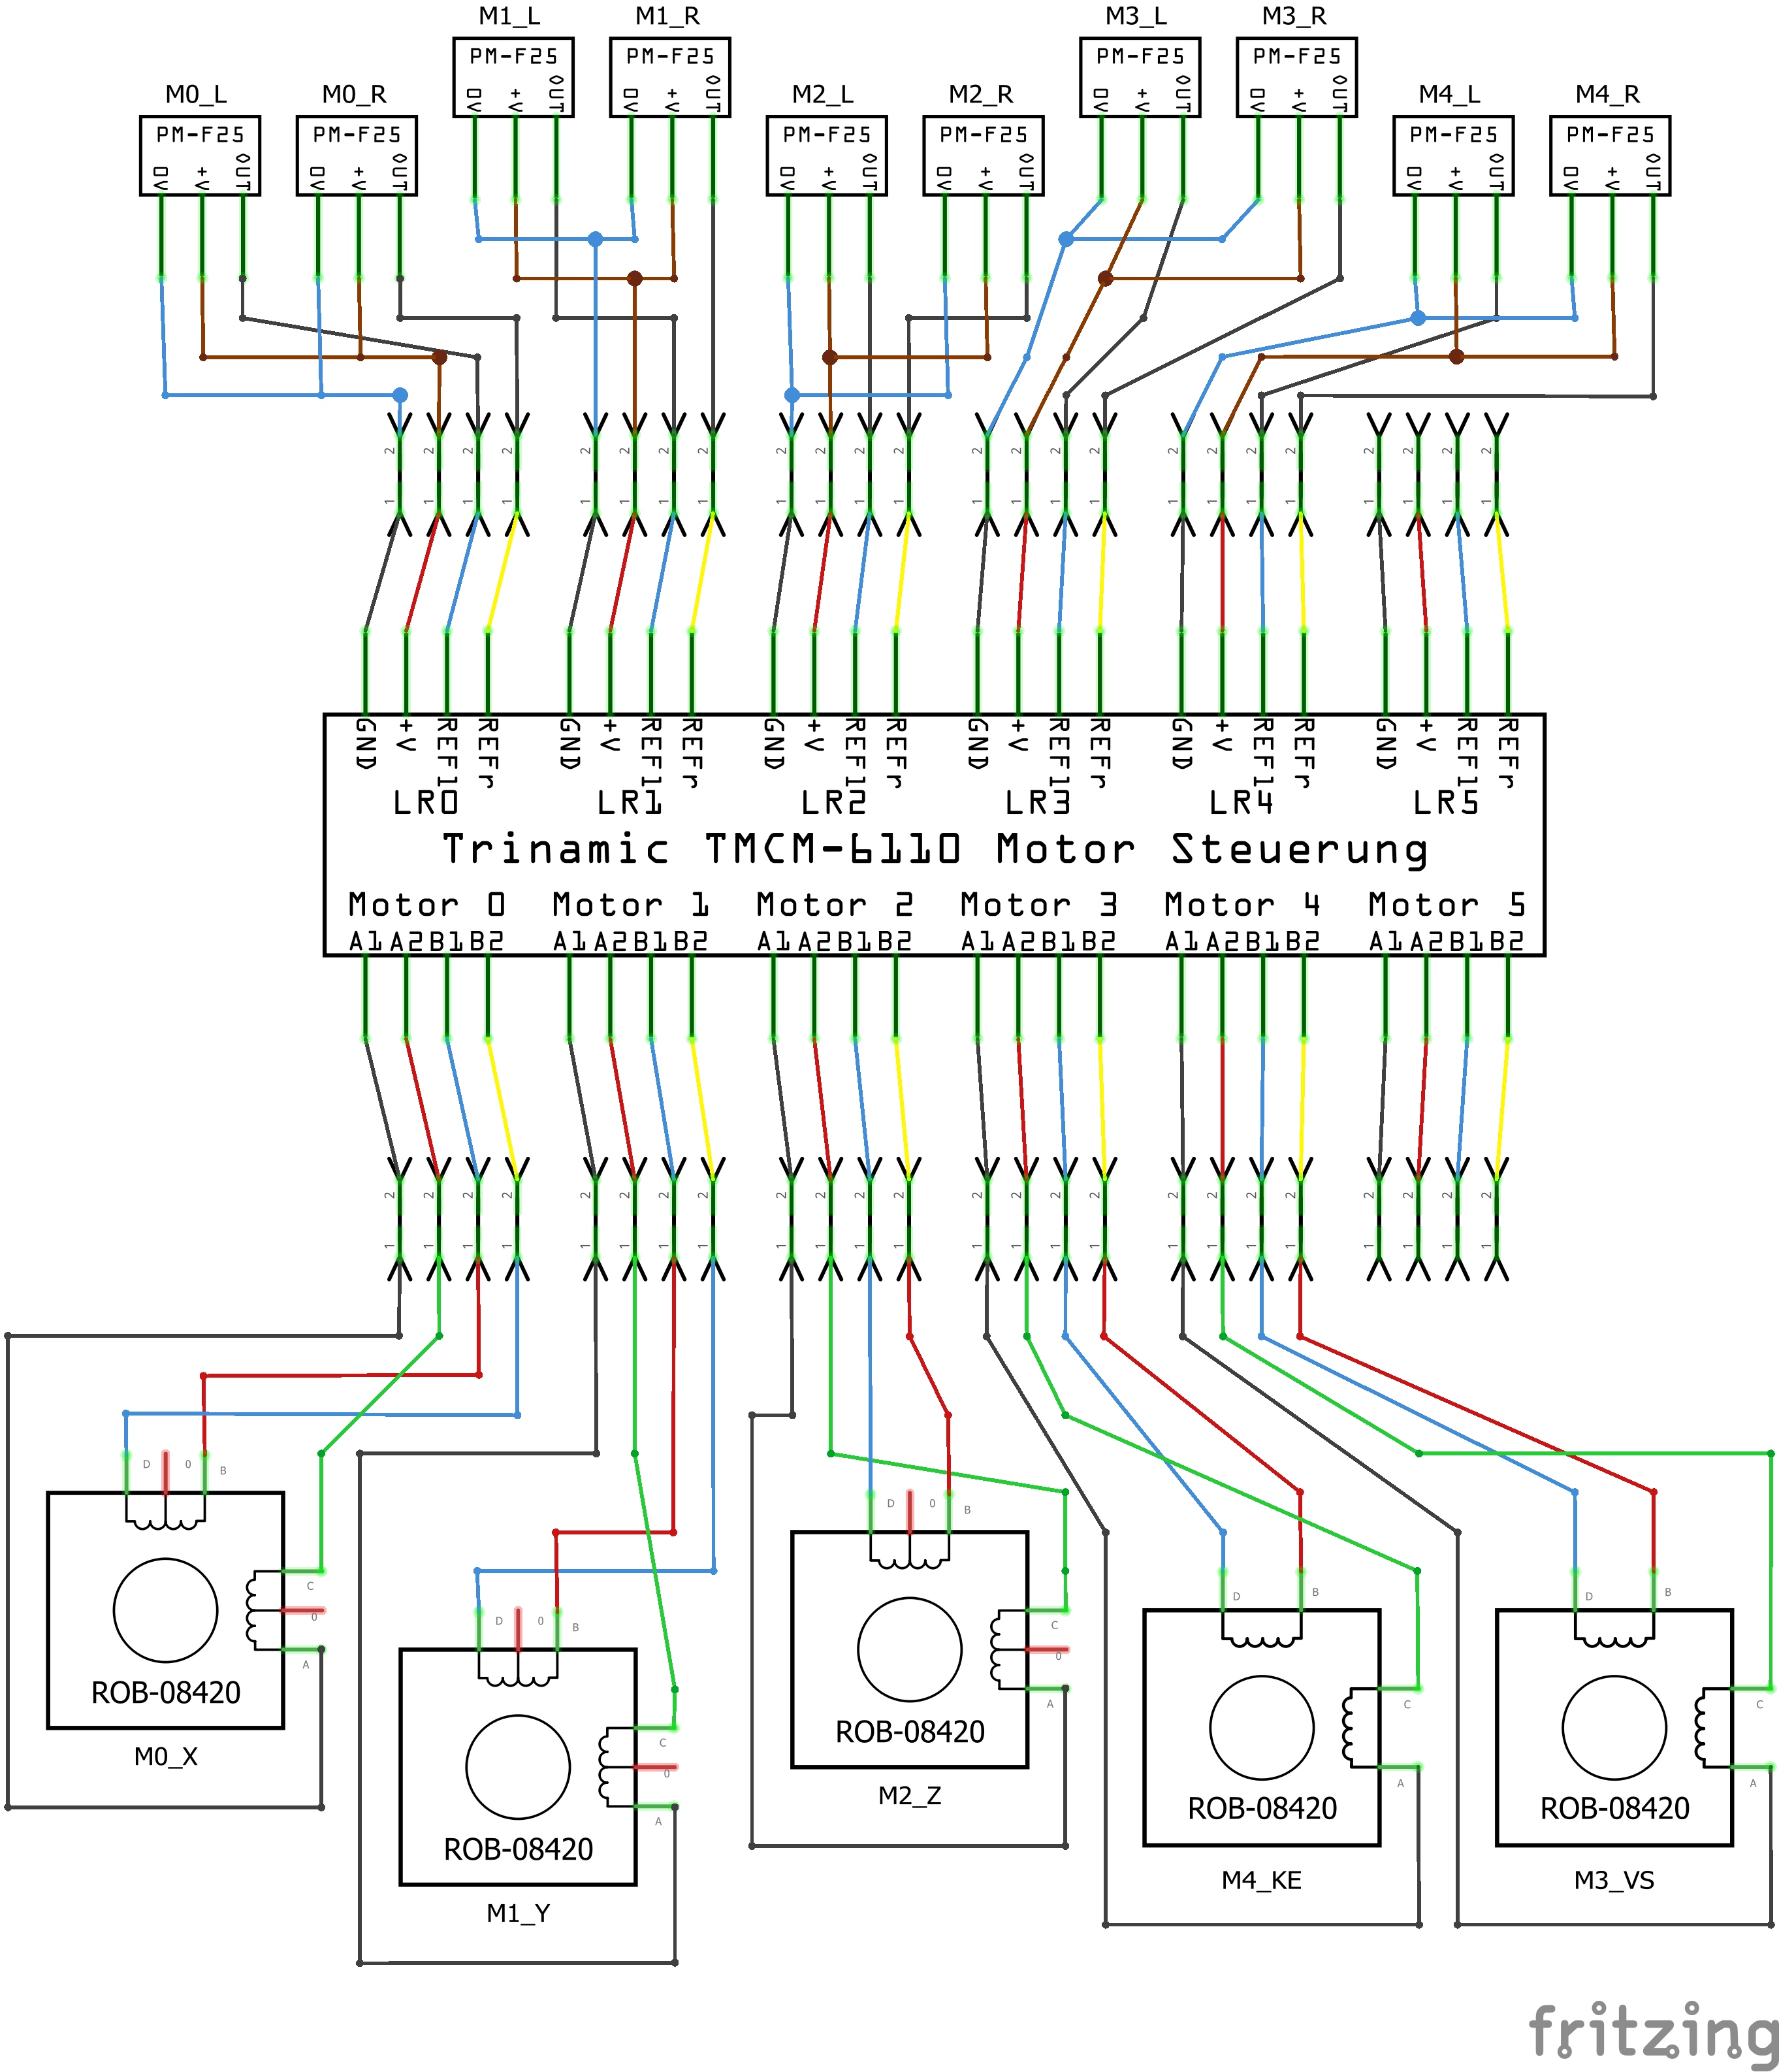
\includegraphics[width=\linewidth]{Anhang/TMCM_Motor_schem.png}
    \caption{Schematische Zeichnung der TMCM-6110 Motor Controller}
    \label{fig:tmcm_m}
\end{figure}

\subsection{TMCM-6110 IO Module}
\begin{figure}[H]
    \centering
    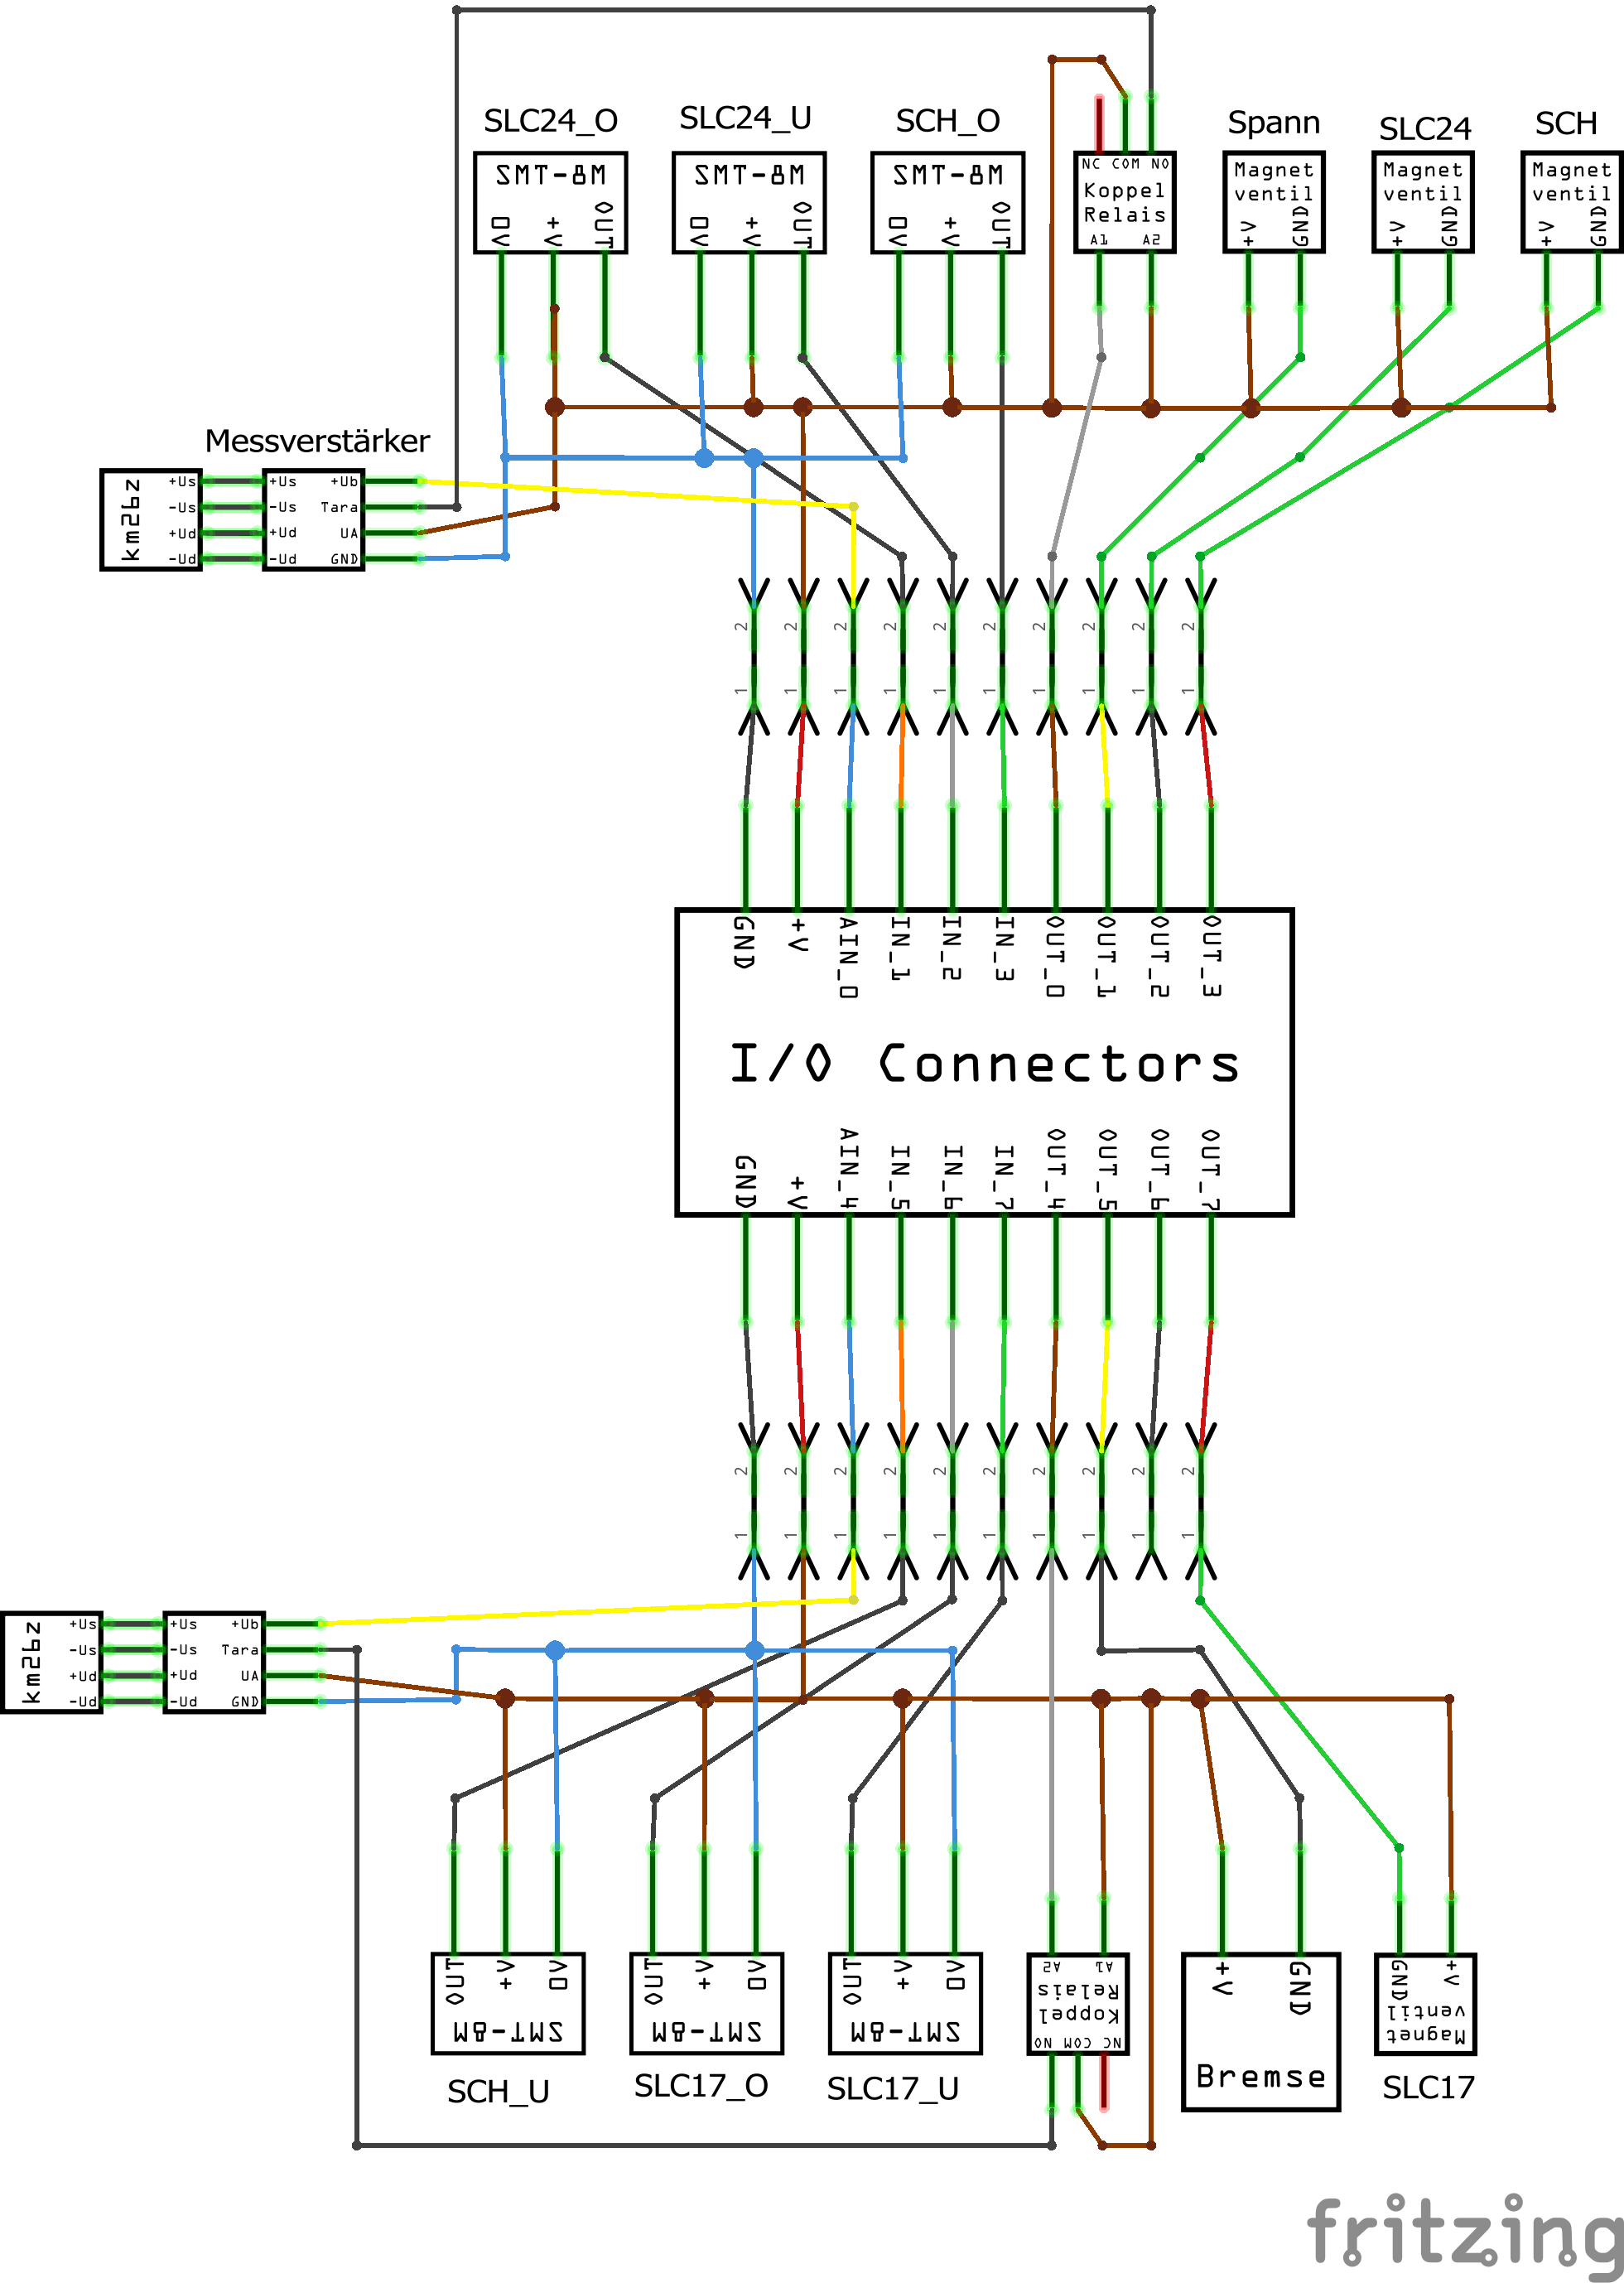
\includegraphics[width=\linewidth]{Anhang/TMCM_IO_schem.png}
    \caption{Schematische Zeichnung der TMCM-6110 IO Module}
    \label{fig:tmcm_io}
\end{figure}

\subsection{WAGO Module}
\begin{figure}[H]
    \centering
    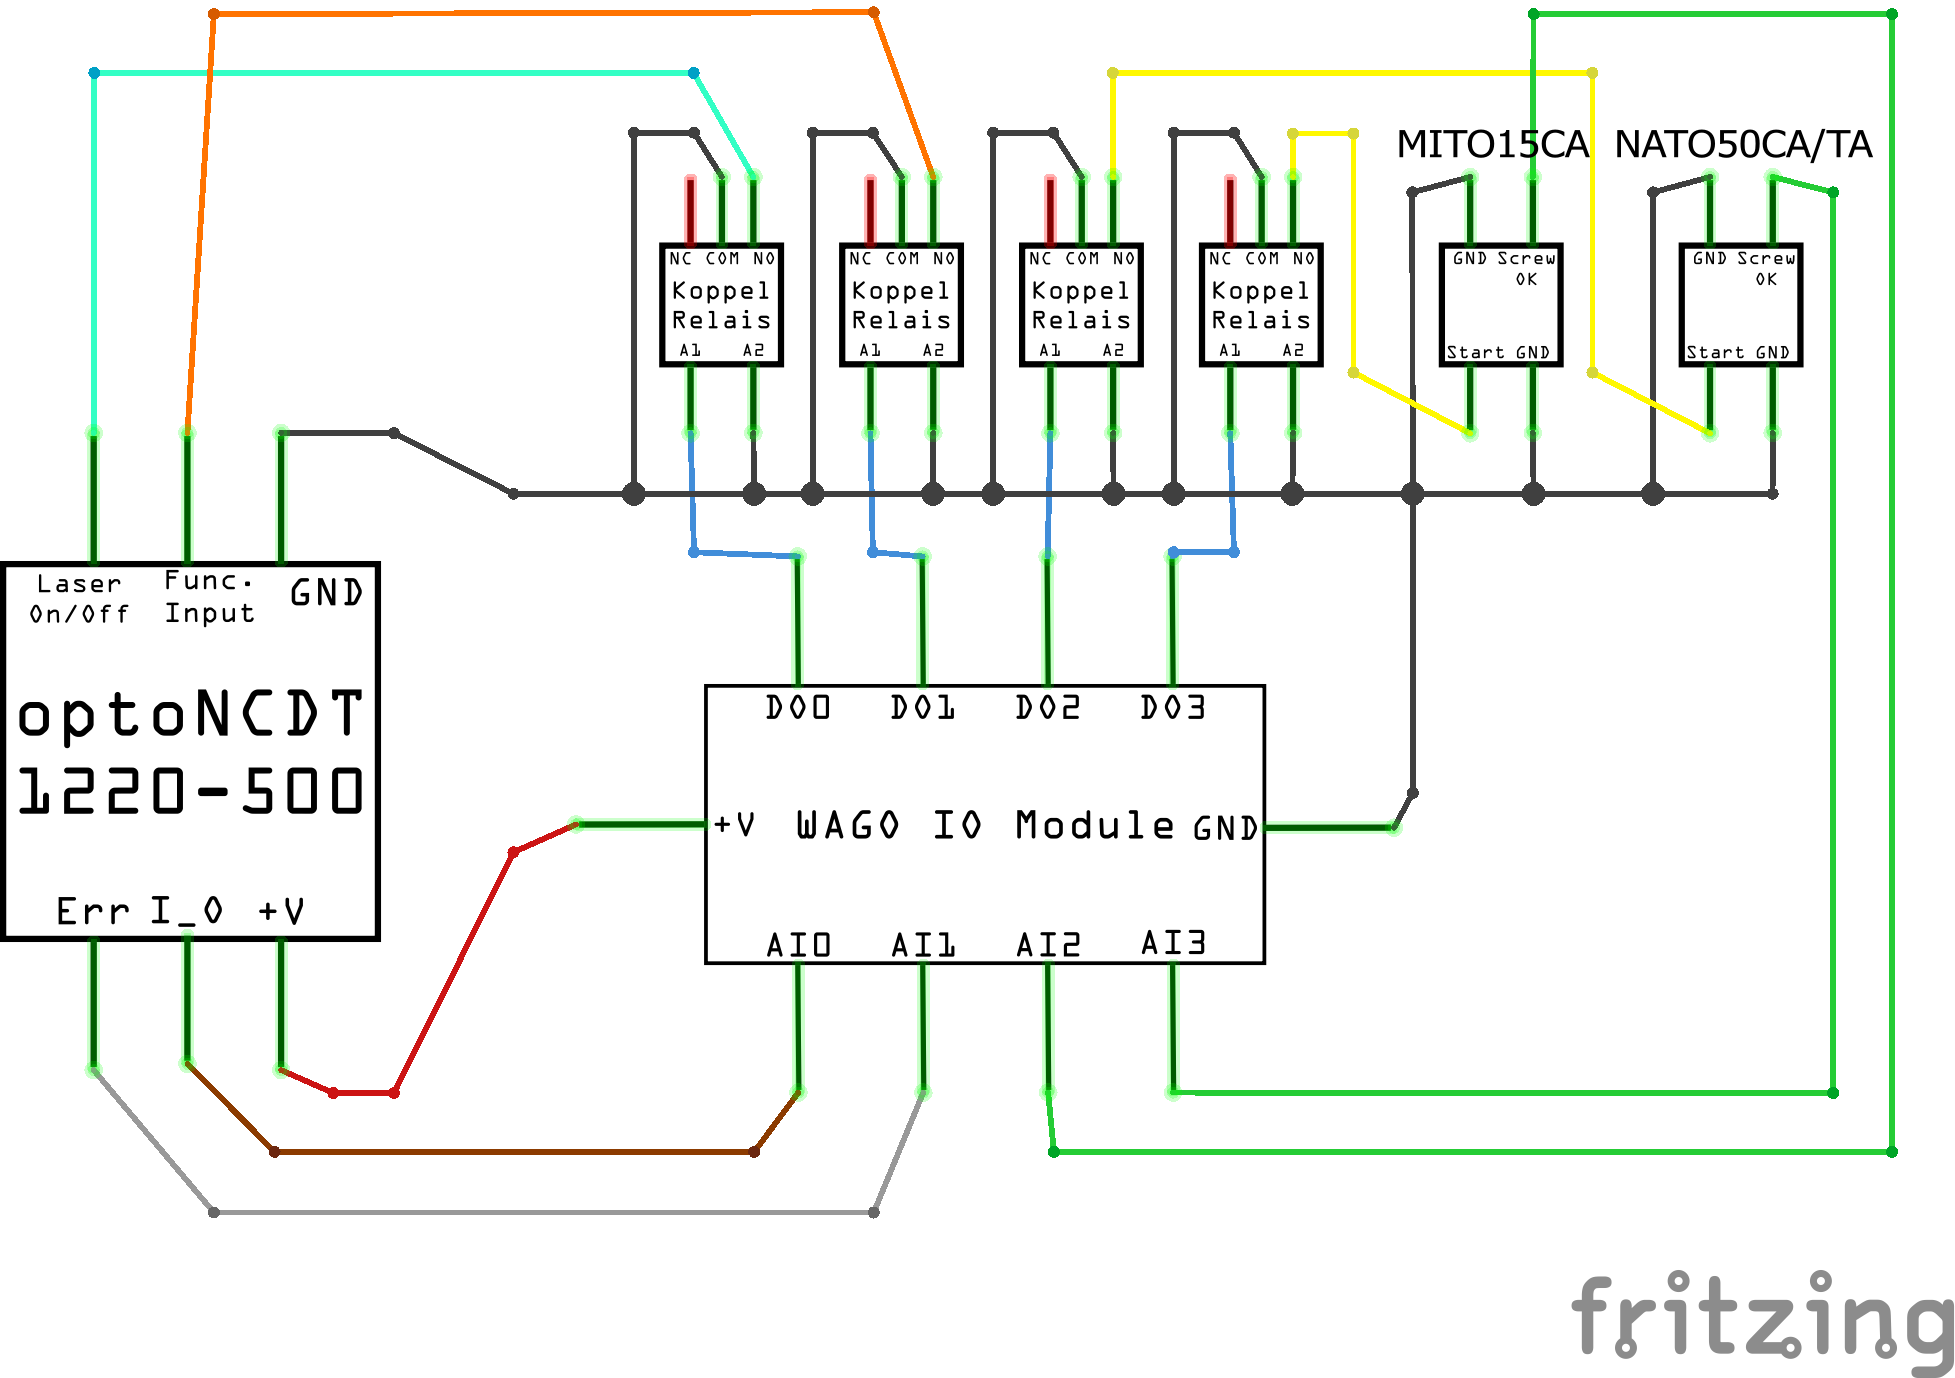
\includegraphics[width=\linewidth]{Anhang/WAGO_schem.png}
    \caption{Schematische Zeichnung der Wago Modul}
    \label{fig:wago}
\end{figure}

\clearpage

\section{Testskripte und Steuerungsprogramme}
\subsection{WAGO-Steuerung}
\subsubsection{WAGO GUI (Visualisierung)}
Das folgende Python-Programm (\texttt{gui.py}) implementiert eine einfache Benutzeroberfläche zur manuellen Ansteuerung digitaler Ausgänge sowie zur Anzeige der Eingangssignale (inkl. Laser-Skalierung). Das Programm wurde ausschließlich für Test- und Inbetriebnahmezwecke im Rahmen der Validierung verwendet.

\begin{lstlisting}[
    style=python-vsc,
    caption={Python GUI zur WAGO-I/O-Ansteuerung (gui.py)},
    label={lst:gui_py}]
# ----------------------------------------------------------
# Simple Tkinter-based graphical user interface for manual testing of a WAGO 750-362 I/O system via Modbus/TCP.
#
# The GUI allows:
# - Manual switching of digital outputs
# - Monitoring of digital and analog inputs
# - Scaling and visualization of a laser triangulation sensor signal
#
# The program was used exclusively for testing and validation purposes
# during the prototype phase of the system.
# ----------------------------------------------------------

import tkinter as tk
from tkinter import ttk, messagebox

# Import WAGO communication backend and configuration
from wago_io import (
    WagoConfig,
    WagoIO,
    DEFAULT_OUTPUT_NAMES,
    DEFAULT_INPUT_NAMES,)

class App(tk.Tk):
    """
    Main application class for the WAGO IO Monitor GUI.
    Handles user interaction, Modbus communication and cyclic polling.
    """

    def __init__(self):
        super().__init__()

        # Window configuration
        self.title("WAGO IO Monitor (Modbus/TCP)")
        self.geometry("600x440")

        # WAGO I/O interface instance
        self.io: WagoIO | None = None
        self.connected = False

        # Tkinter timer ID for cyclic polling
        self.after_id: str | None = None

        # Build the user interface
        self._build_ui()

    def _build_ui(self):
        """
        Creates all GUI elements (connection settings, IO display, buttons).
        """
        frm = ttk.Frame(self, padding=10)
        frm.pack(fill="both", expand=True)

        # --------------------------------------------------
        # Connection settings
        # --------------------------------------------------
        conn = ttk.LabelFrame(frm, text="Connection", padding=10)
        conn.pack(fill="x")

        ttk.Label(conn, text="IP:").grid(row=0, column=0, sticky="w")
        self.ip_var = tk.StringVar(value="192.168.1.31")
        ttk.Entry(conn, textvariable=self.ip_var, width=18).grid(
            row=0, column=1, sticky="w", padx=6)

        ttk.Label(conn, text="Port:").grid(row=0, column=2, sticky="w")
        self.port_var = tk.StringVar(value="502")
        ttk.Entry(conn, textvariable=self.port_var, width=6).grid(
            row=0, column=3, sticky="w", padx=6)

        self.btn_connect = ttk.Button(conn, text="Connect", command=self.on_connect)
        self.btn_connect.grid(row=0, column=4, padx=6)

        self.btn_disconnect = ttk.Button(
            conn, text="Disconnect", command=self.on_disconnect, state="disabled")
        self.btn_disconnect.grid(row=0, column=5)

        self.status_var = tk.StringVar(value="Disconnected")
        ttk.Label(conn, textvariable=self.status_var).grid(
            row=1, column=0, columnspan=6, sticky="w", pady=(8, 0))

        # --------------------------------------------------
        # Laser sensor scaling configuration
        # --------------------------------------------------
        laser = ttk.LabelFrame(frm, text="Laser scaling (4..20 mA -> mm)", padding=10)
        laser.pack(fill="x", pady=(10, 0))

        ttk.Label(laser, text="Start mm @4mA:").grid(row=0, column=0, sticky="w")
        self.laser_start_var = tk.StringVar(value="100.0")
        ttk.Entry(laser, textvariable=self.laser_start_var, width=10).grid(
            row=0, column=1, sticky="w", padx=6)

        ttk.Label(laser, text="End mm @20mA:").grid(row=0, column=2, sticky="w")
        self.laser_end_var = tk.StringVar(value="600.0")
        ttk.Entry(laser, textvariable=self.laser_end_var, width=10).grid(
            row=0, column=3, sticky="w", padx=6)

        ttk.Label(laser, text="AI FS counts:").grid(row=0, column=4, sticky="w")
        self.fs_var = tk.StringVar(value="32767")
        ttk.Entry(laser, textvariable=self.fs_var, width=8).grid(
            row=0, column=5, sticky="w", padx=6)

        # --------------------------------------------------
        # IO panels
        # --------------------------------------------------
        pan = ttk.Frame(frm)
        pan.pack(fill="both", expand=True, pady=(10, 0))

        # Digital Outputs
        out_box = ttk.LabelFrame(pan, text="Outputs (coils)", padding=10)
        out_box.pack(side="left", fill="both", expand=True, padx=(0, 5))

        self.out_vars: list[tk.IntVar] = []
        for i, name in enumerate(DEFAULT_OUTPUT_NAMES):
            v = tk.IntVar(value=0)
            self.out_vars.append(v)

            row = ttk.Frame(out_box)
            row.pack(fill="x", pady=2)

            ttk.Label(
                row, text=f"DO{i}: {name}", wraplength=260
            ).pack(side="left", fill="x", expand=True)

            ttk.Checkbutton(
                row,
                variable=v,
                command=lambda idx=i: self.on_toggle_output(idx)
            ).pack(side="right")

        btn_row = ttk.Frame(out_box)
        btn_row.pack(fill="x", pady=(8, 0))
        ttk.Button(btn_row, text="All OFF", command=self.all_off).pack(side="left", padx=(0, 6))
        ttk.Button(btn_row, text="All ON", command=self.all_on).pack(side="left")

        # Analog Inputs
        in_box = ttk.LabelFrame(pan, text="Inputs (input registers)", padding=10)
        in_box.pack(side="left", fill="both", expand=True, padx=(5, 0))

        self.in_labels: list[ttk.Label] = []
        for i, name in enumerate(DEFAULT_INPUT_NAMES):
            lbl = ttk.Label(in_box, text=f"AI{i}: {name} = -")
            lbl.pack(anchor="w", pady=2)
            self.in_labels.append(lbl)

        self.laser_label = ttk.Label(
            in_box,
            text="Laser distance (mm) = -",
            font=("Segoe UI", 10, "bold"))
        self.laser_label.pack(anchor="w", pady=(10, 2))

    def _apply_cfg_from_ui(self) -> WagoConfig:
        """
        Reads configuration values from the GUI and returns a WagoConfig object.
        """
        return WagoConfig(
            host=self.ip_var.get().strip(),
            port=int(self.port_var.get().strip()),
            laser_start_mm=float(self.laser_start_var.get().strip()),
            laser_end_mm=float(self.laser_end_var.get().strip()),
            ai_fullscale_counts=int(self.fs_var.get().strip()),)

    def on_connect(self):
        """
        Establishes the Modbus/TCP connection to the WAGO controller.
        """
        if self.connected:
            return

        try:
            cfg = self._apply_cfg_from_ui()
            self.io = WagoIO(cfg)
            ok = self.io.connect()
            if not ok:
                raise RuntimeError("Modbus connect failed.")
        except Exception as e:
            messagebox.showerror("Connect error", str(e))
            self.io = None
            return

        self.connected = True
        self.status_var.set(f"Connected to {self.io.cfg.host}:{self.io.cfg.port}")
        self.btn_connect.config(state="disabled")
        self.btn_disconnect.config(state="normal")

        # Start cyclic polling
        self._poll()

    def on_disconnect(self):
        """
        Disconnects from the WAGO controller and stops polling.
        """
        self._stop_poll()
        if self.io:
            try:
                self.io.close()
            except Exception:
                pass
        self.io = None
        self.connected = False
        self.status_var.set("Disconnected")
        self.btn_connect.config(state="normal")
        self.btn_disconnect.config(state="disabled")

    def _stop_poll(self):
        """
        Stops the cyclic polling loop.
        """
        if self.after_id is not None:
            try:
                self.after_cancel(self.after_id)
            except Exception:
                pass
            self.after_id = None

    def _poll(self):
        """
        Periodically reads inputs and outputs from the WAGO controller and updates the GUI.
        """
        if not self.connected or not self.io:
            return

        try:
            # Update configuration dynamically (laser scaling)
            try:
                new_cfg = self._apply_cfg_from_ui()
                self.io.cfg.laser_start_mm = new_cfg.laser_start_mm
                self.io.cfg.laser_end_mm = new_cfg.laser_end_mm
                self.io.cfg.ai_fullscale_counts = new_cfg.ai_fullscale_counts
            except Exception:
                pass

            # Read digital outputs
            outs = self.io.read_outputs()
            for i, val in enumerate(outs):
                if self.out_vars[i].get() != val:
                    self.out_vars[i].set(val)

            # Read analog inputs
            ins = self.io.read_inputs()
            for i in range(4):
                raw = ins.get(f"AI{i}_raw", float("nan"))
                mA = ins.get(f"AI{i}_mA", float("nan"))
                self.in_labels[i].config(
                    text=f"AI{i}: {DEFAULT_INPUT_NAMES[i]} = raw {raw:.0f} | {mA:.3f} mA")

            # Display scaled laser distance
            self.laser_label.config(
                text=f"Laser distance (mm) = {ins['Laser_mm']:.3f} mm   ({ins['Laser_mA']:.3f} mA)")

            self.status_var.set(f"Connected to {self.io.cfg.host}:{self.io.cfg.port}")

        except Exception as e:
            self.status_var.set(f"Error: {e}")

        # Poll at 5 Hz
        self.after_id = self.after(200, self._poll)

    def on_toggle_output(self, idx: int):
        """
        Writes a single digital output to the WAGO controller.
        """
        if not self.connected or not self.io:
            return
        try:
            val = int(self.out_vars[idx].get())
            self.io.set_output(idx, val)
        except Exception as e:
            messagebox.showerror("Write error", str(e))

    def all_off(self):
        """
        Switches all digital outputs OFF.
        """
        if not self.connected or not self.io:
            return
        try:
            for i in range(len(self.out_vars)):
                self.out_vars[i].set(0)
                self.io.set_output(i, 0)
        except Exception as e:
            messagebox.showerror("Write error", str(e))

    def all_on(self):
        """
        Switches all digital outputs ON.
        """
        if not self.connected or not self.io:
            return
        try:
            for i in range(len(self.out_vars)):
                self.out_vars[i].set(1)
                self.io.set_output(i, 1)
        except Exception as e:
            messagebox.showerror("Write error", str(e))


if __name__ == "__main__":
    # Start the GUI application
    App().mainloop()
\end{lstlisting}

\clearpage

\subsubsection{WAGO Backend (Prozesslogik)}
Das Backend-Programm bildet die grundlegende Prozesslogik der Anlage ab.
Hierzu zählen die Verknüpfung von Sensorsignalen, Sicherheitsabfragen sowie die logische Freigabe der Aktoren während der Tests.

\begin{lstlisting}[
    style=python-vsc,
    caption={WAGO Backend Code},
    label={lst:wago_backend}]
# ----------------------------------------------------------
# Helper module for WAGO 750-362 communication via Modbus/TCP.
#
# Hardware mapping used in the prototype:
# - Digital outputs (coils):     WAGO 750-531
# - Analog inputs (input regs):  2x WAGO 750-466  -> 4 channels total
# - Laser sensor: micro-epsilon optoNCDT 1220-500 (4..20 mA corresponds to 100..600 mm)
#
# Purpose:
# This module was used for manual testing and validation of I/O signals.
# It provides simple read/write functions and a conversion for the laser current signal.
# ----------------------------------------------------------

from dataclasses import dataclass
from typing import Dict, List, Optional

from pymodbus.client import ModbusTcpClient


@dataclass
class WagoConfig:
    """
    Configuration parameters for Modbus/TCP and the I/O mapping.
    Adjust start addresses/counts if the WAGO I/O order changes.
    """
    host: str = "192.168.1.31"
    port: int = 502

    # Digital outputs (WAGO 750-531)
    # Coils start address and number of outputs used in the project.
    do_coil_start: int = 0
    do_count: int = 4

    # Analog inputs (2x WAGO 750-466)
    # Input register start address and number of analog channels (4 total).
    ai_inputreg_start: int = 0
    ai_count: int = 4

    # Full-scale raw counts of the analog module (typical: 32767).
    ai_fullscale_counts: int = 32767

    # Laser sensor scaling
    # For optoNCDT 1220-500: 4 mA -> 100 mm and 20 mA -> 600 mm
    laser_start_mm: float = 100.0     # value at 4 mA
    laser_end_mm: float = 600.0       # value at 20 mA
    laser_ai_channel: int = 0         # which AI channel is used for the laser signal (AI0)


class WagoIO:
    """
    Lightweight Modbus/TCP interface for reading WAGO inputs and writing outputs.
    """

    def __init__(self, cfg: WagoConfig):
        self.cfg = cfg
        self.client: Optional[ModbusTcpClient] = None

    # ------------------------------------------------------
    # Connection handling
    # ------------------------------------------------------

    def connect(self) -> bool:
        """
        Create a Modbus/TCP client and connect to the WAGO controller.
        Returns True on successful connection.
        """
        self.client = ModbusTcpClient(
            host=self.cfg.host,
            port=self.cfg.port,
            timeout=2.0,)
        return bool(self.client.connect())

    def close(self) -> None:
        """
        Close the Modbus connection (if open).
        """
        if self.client:
            self.client.close()
        self.client = None

    def _ensure(self) -> ModbusTcpClient:
        """
        Internal helper: ensures that a connection exists.
        """
        if not self.client:
            raise RuntimeError("Not connected")
        return self.client

    # ------------------------------------------------------
    # Digital outputs (coils)
    # ------------------------------------------------------
    def read_outputs(self) -> List[int]:
        """
        Read the configured digital output states (coils).
        Returns a list with 0/1 values.
        """
        c = self._ensure()
        rr = c.read_coils(
            address=self.cfg.do_coil_start,
            count=self.cfg.do_count,)
        if rr.isError():
            raise RuntimeError(f"read_coils error: {rr}")

        # rr.bits contains booleans; convert to integer 0/1
        return [1 if b else 0 for b in rr.bits[:self.cfg.do_count]]

    def set_output(self, index: int, value: int) -> None:
        """
        Write one digital output (coil) by index.
        index: 0..do_count-1
        value: 0/1 (internally cast to bool)
        """
        if index < 0 or index >= self.cfg.do_count:
            raise ValueError("Output index out of range")

        c = self._ensure()
        rr = c.write_coil(
            address=self.cfg.do_coil_start + index,
            value=bool(value),)
        if rr.isError():
            raise RuntimeError(f"write_coil error: {rr}")

    # ------------------------------------------------------
    # Analog inputs (input registers)
    # ------------------------------------------------------
    def read_inputs_raw(self) -> List[int]:
        """
        Read analog input registers (raw counts).
        Returns a list of integer register values.
        """
        c = self._ensure()
        rr = c.read_input_registers(
            address=self.cfg.ai_inputreg_start,
            count=self.cfg.ai_count,)
        if rr.isError():
            raise RuntimeError(f"read_input_registers error: {rr}")

        return rr.registers[:self.cfg.ai_count]

    def raw_to_mA(self, raw: int) -> float:
        """
        Convert raw analog counts to an approximate current in mA.
        The conversion is scaled to 0..20 mA based on ai_fullscale_counts.
        """
        fs = float(self.cfg.ai_fullscale_counts)

        # Clamp raw signal to a valid range
        raw_f = max(0.0, min(float(raw), fs))

        # Map counts to 0..20 mA (sufficient for validation use)
        return (raw_f / fs) * 20.0

    def mA_to_distance_mm(self, mA: float) -> float:
        """
        Convert current (mA) to distance (mm) for the optoNCDT laser sensor.
        Uses linear scaling: 4..20 mA -> laser_start_mm..laser_end_mm.
        Values outside 4..20 mA are clamped.
        """
        x = (mA - 4.0) / 16.0
        x = max(0.0, min(1.0, x))
        return self.cfg.laser_start_mm + x * (
            self.cfg.laser_end_mm - self.cfg.laser_start_mm)

    def read_inputs(self) -> Dict[str, float]:
        """
        Read all analog inputs and return a dictionary with:
        - AIi_raw, AIi_mA for each channel
        - Laser_raw, Laser_mA, Laser_mm (derived from the configured laser channel)
        """
        raws = self.read_inputs_raw()
        currents = [self.raw_to_mA(r) for r in raws]

        # Extract laser channel values
        laser_raw = raws[self.cfg.laser_ai_channel]
        laser_mA = currents[self.cfg.laser_ai_channel]
        laser_mm = self.mA_to_distance_mm(laser_mA)

        # Build result dictionary (easy to use in GUI/logging)
        data: Dict[str, float] = {}
        for i, (r, mA) in enumerate(zip(raws, currents)):
            data[f"AI{i}_raw"] = float(r)
            data[f"AI{i}_mA"] = float(mA)

        data["Laser_raw"] = float(laser_raw)
        data["Laser_mA"] = float(laser_mA)
        data["Laser_mm"] = float(laser_mm)
        return data

# ----------------------------------------------------------
# Optional signal names (used by GUI and for consistent logging)
# ----------------------------------------------------------

DEFAULT_OUTPUT_NAMES = [
    "Laser Beam On/Off",
    "Laser Function Input",
    "Kolver NATO Start",
    "Kolver MITO Start",]

DEFAULT_INPUT_NAMES = [
    "Laser I_OUT",
    "Laser Error",
    "MITO SCREW_OK",
    "NATO SCREW_OK",]

\end{lstlisting}

\clearpage
\subsection{TMCM-6110 Testskript (TMCL-IDE)}
Das nachfolgende TMCL-Skript wurde im TMCL-IDE erstellt und diente zur Initialisierung sowie zum Test der einzelnen Linearachsen. Die Skripte wurden ausschließlich zu Validierungs- und Inbetriebnahmezwecken verwendet.

\begin{lstlisting}[
    style=tmcl-vsc,
    caption={TMCL-Testskript},
    label={lst:tmcl_test}]
// ---------------------------------------------------------
// TMCL Initialisierungsskript fuer Trinamic TMCM-6110
// Zweck:
// - Parametrierung der Achsen X, Y, Z, Keileinpressen, Vorspannen
// - Einfache Sicherheitsabschaltung ueber digitalen Eingang
// Einsatz: Inbetriebnahme und Validierung
// ---------------------------------------------------------

// ----------------------
// Allgemeine Einstellungen
// ----------------------

// Pull-Up Konfiguration digitale Eingaenge
// 0 = keine Pull-Ups
// 1 = Pull-Ups Achse 0-2
// 2 = Pull-Ups Achse 3-5
// 3 = Pull-Ups Achse 0-5
SGP 77, 0, 1        // Auto-Start aktivieren


// =========================================================
// Achse 1 (Kanal 0) - X-Achse
// =========================================================
SAP   4, 0, 2000    // maximale Positioniergeschwindigkeit
SAP   5, 0, 1000    // maximale Beschleunigung
SAP   6, 0, 200     // maximaler Motorstrom
SAP   7, 0, 30      // Haltestrom
SAP  12, 0, 0       // rechter Endschalter deaktiviert
SAP  13, 0, 0       // linker Endschalter deaktiviert
SAP 138, 0, 0       // Positioniermodus
SAP 140, 0, 5       // Mikroschrittauflosung
SAP 153, 0, 5       // Ramp Divider
SAP 154, 0, 5       // Pulse Divider
SAP 194, 0, 1000    // Referenzfahrgeschwindigkeit


// =========================================================
// Achse 2 (Kanal 1) - Y-Achse
// =========================================================
SAP   4, 1, 2000
SAP   5, 1, 1000
SAP   6, 1, 150
SAP   7, 1, 50
SAP  12, 1, 0
SAP  13, 1, 0
SAP 138, 1, 2       // Geschwindigkeitsmodus
SAP 150, 1, 1       // Endschalter Power-Down aktiv
SAP 140, 1, 4
SAP 153, 1, 5
SAP 154, 1, 5
SAP 194, 1, 2000


// =========================================================
// Achse 3 (Kanal 2) - Z-Achse
// =========================================================
SAP   4, 2, 2000
SAP   5, 2, 1000
SAP   6, 2, 150
SAP   7, 2, 30
SAP  12, 2, 0
SAP  13, 2, 0
SAP 138, 2, 0
SAP 140, 2, 4
SAP 153, 2, 5
SAP 154, 2, 5
SAP 194, 2, 2000


// =========================================================
// Achse 4 (Kanal 3) - Keileinpressen
// =========================================================
SAP   4, 3, 2000
SAP   5, 3, 1500
SAP   6, 3, 156
SAP   7, 3, 30
SAP  12, 3, 0
SAP  13, 3, 0
SAP 138, 3, 2
SAP 140, 3, 5
SAP 153, 3, 6
SAP 154, 3, 4
SAP 194, 3, 1200


// =========================================================
// Achse 5 (Kanal 4) - Vorspannen
// =========================================================
SAP   4, 4, 2000
SAP   5, 4, 200
SAP   6, 4, 160
SAP   7, 4, 30
SAP  12, 4, 0
SAP  13, 4, 0
SAP 138, 4, 0
SAP 140, 4, 6
SAP 153, 4, 5
SAP 154, 4, 5
SAP 194, 4, 1500


// =========================================================
// Sicherheitsueberwachung
// =========================================================

LOOP:
    GIO 8, 1            // digitalen Eingang lesen
    COMP 200            // mit Schwellwert vergleichen
    JC LT, MOTORSTOP    // wenn kleiner 200 -> Motorstop
    JA LOOP             // sonst weiter pruefen


// =========================================================
// Not-Stopp Routine
// =========================================================

MOTORSTOP:
    MST 0
    MST 1
    MST 2
    MST 3
    MST 4
    MST 5
    JA LOOP

STOP
\end{lstlisting}